\chapter[Lavrentiy Zagoskin’s Contributions to the Study of Alaska Native Place Names]{\vspace{-25pt}“From this point...the river changes its name again”: Lavrentiy Zagoskin’s Contributions to the Study of Alaska Native Place Names}
%\chaptermark{“From this point...the river changes its name again”: Lavrentiy Zagoskin’s Contributions to the Study of Alaska Native Place Names}
%% make sure long title appears in toc
\sethandle{10125/24839}



% Author last name as it appears in the header
\def\authorlast{Pratt}


\renewcommand{\beginchapter}{\pageref{pratt-ch-begin}}
\renewcommand{\finishchapter}{\pageref{pratt-ch-end}}
\label{pratt-ch-begin}



\thispagestyle{firststyle}

\chapauth{Kenneth L. Pratt}
\affiliation{Bureau of Indian Affairs, ANCSA Program}

\authortoc{Kenneth L. Pratt}

The accounts of Euroamerican explorers are the earliest sources of Native place names in Alaska but those accounts often receive inadequate attention from researchers, and the same is true of contextual issues related to the data they contain. Comprehensive literature searches for previously recorded place names in one’s geographical area of concern should be an essential component of any research project focused on Native place names. That often is not the case, however---usually due to indifference, tight research schedules, a primary focus on information held by today’s elders (e.g., Fienup-Riordan 2014), or assumptions of authoritative and timeless knowledge of traditional landscapes (including place names) among contemporary Native peoples.\footnote{It may not be possible to reliably quantify the process but some degree of loss in place names knowledge has likely occurred in every human generation. For Alaska’s indigenous populations, it stands to reason that the rate of such generational losses would increase in step with cultural changes that reduce its members’ time on the land. In this author’s opinion, regardless of which area of Alaska is under discussion, today’s indigenous peoples arguably possess less knowledge of place names in their traditional territories than did any previous indigenous generations.}

Typically, the most problematic element of thorough literature searches involves early historical sources—many authors of which either disregarded Native place names or provided so little contextual information about those they did report that correlating them with fixed points on the land can be extremely difficult. Carefully reviewing historical sources is not quick or easy, but the recovery of obscure, long-lost place names that can expand knowledge of local or regional Native history is one of the possible rewards. The potential value of such reviews is highlighted by the following discussion about the 1842-1844 expedition of Russian Naval Lieutenant Lavrentiy Zagoskin (1967; Figure~\ref{pratt-fig1}), an explorer who paid very close attention to Alaska Native place names. The map of Zagoskin’s expedition (Figure~\ref{pratt-fig2}) clearly hints at this fact.

\begin{figure}[ht]
    \centering
    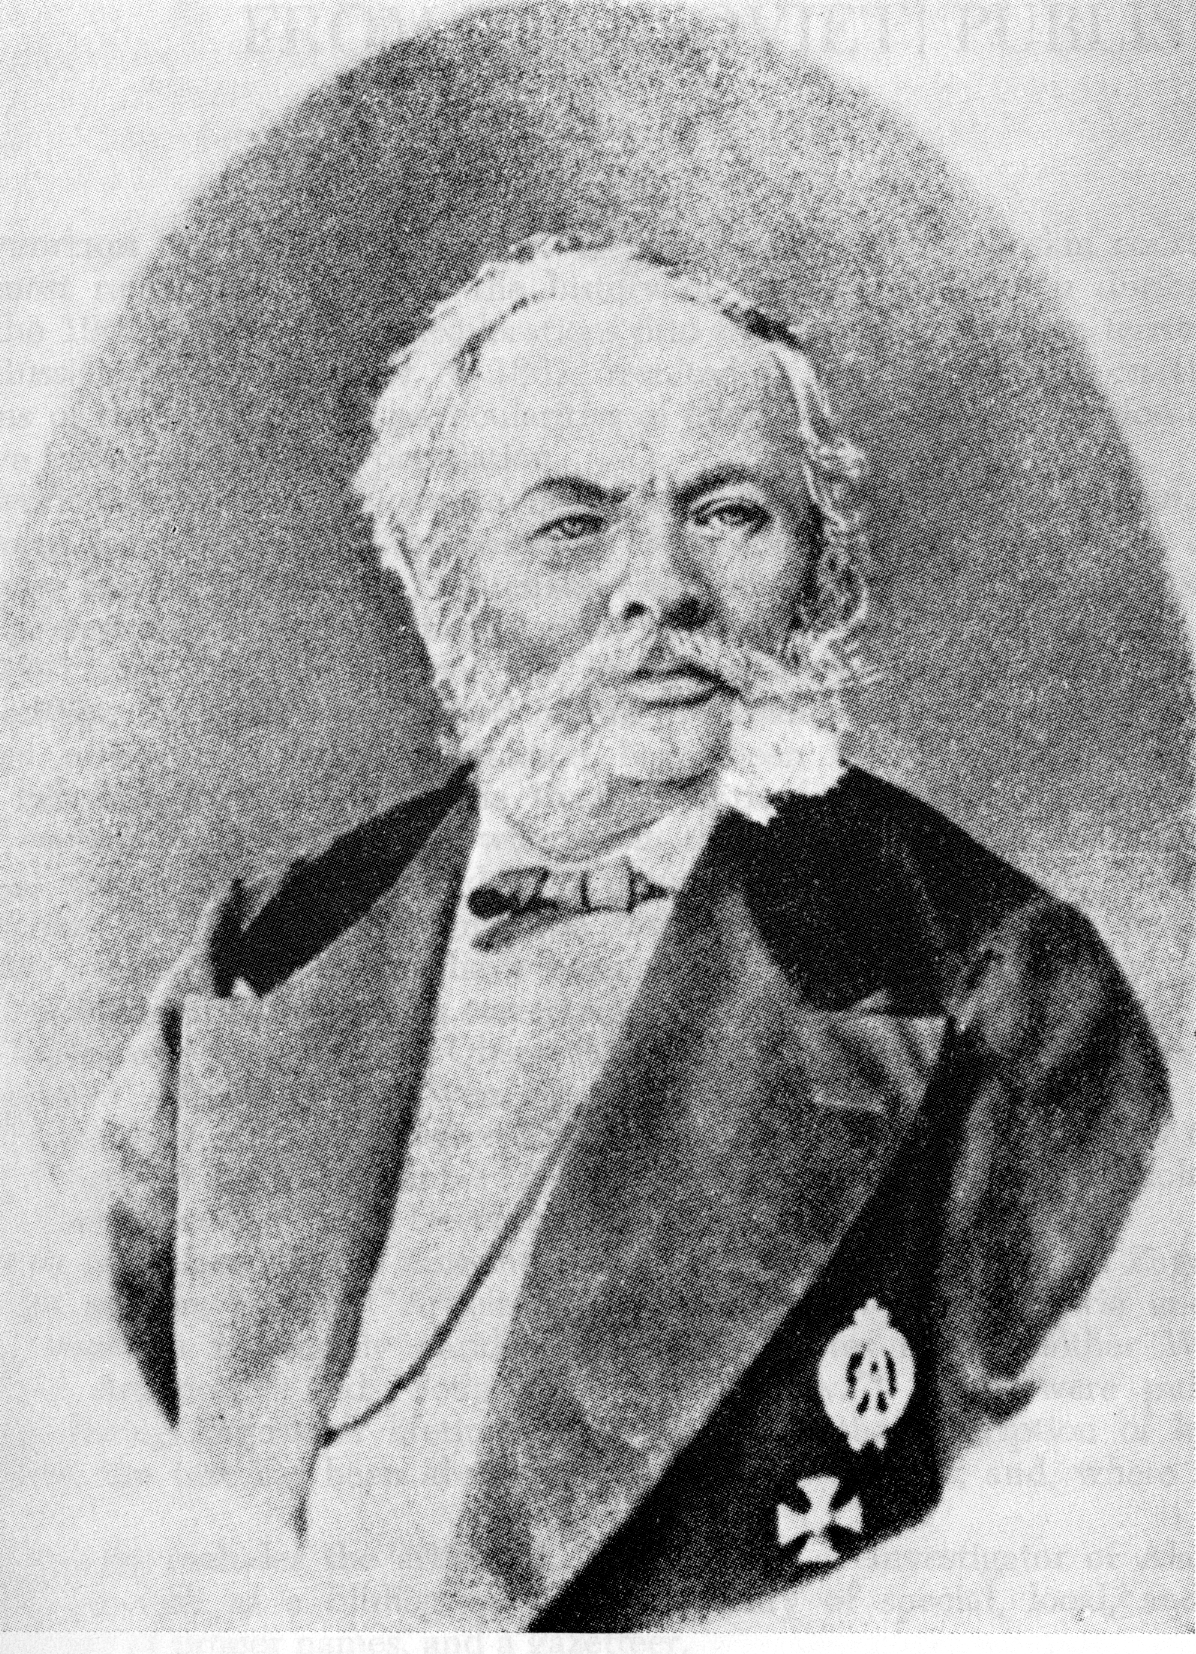
\includegraphics[width=0.6\textwidth]{figures/pratt-fig1}
    \caption{Portrait of Lavrentiy A. Zagoskin (from Chernenko et al. 1956 [Frontispiece])}
    \label{pratt-fig1}
\end{figure}

%\begin{center}
%    \begin{sideways}%[htbp]
%         \begin{minipage}{0.92\linewidth}
%                    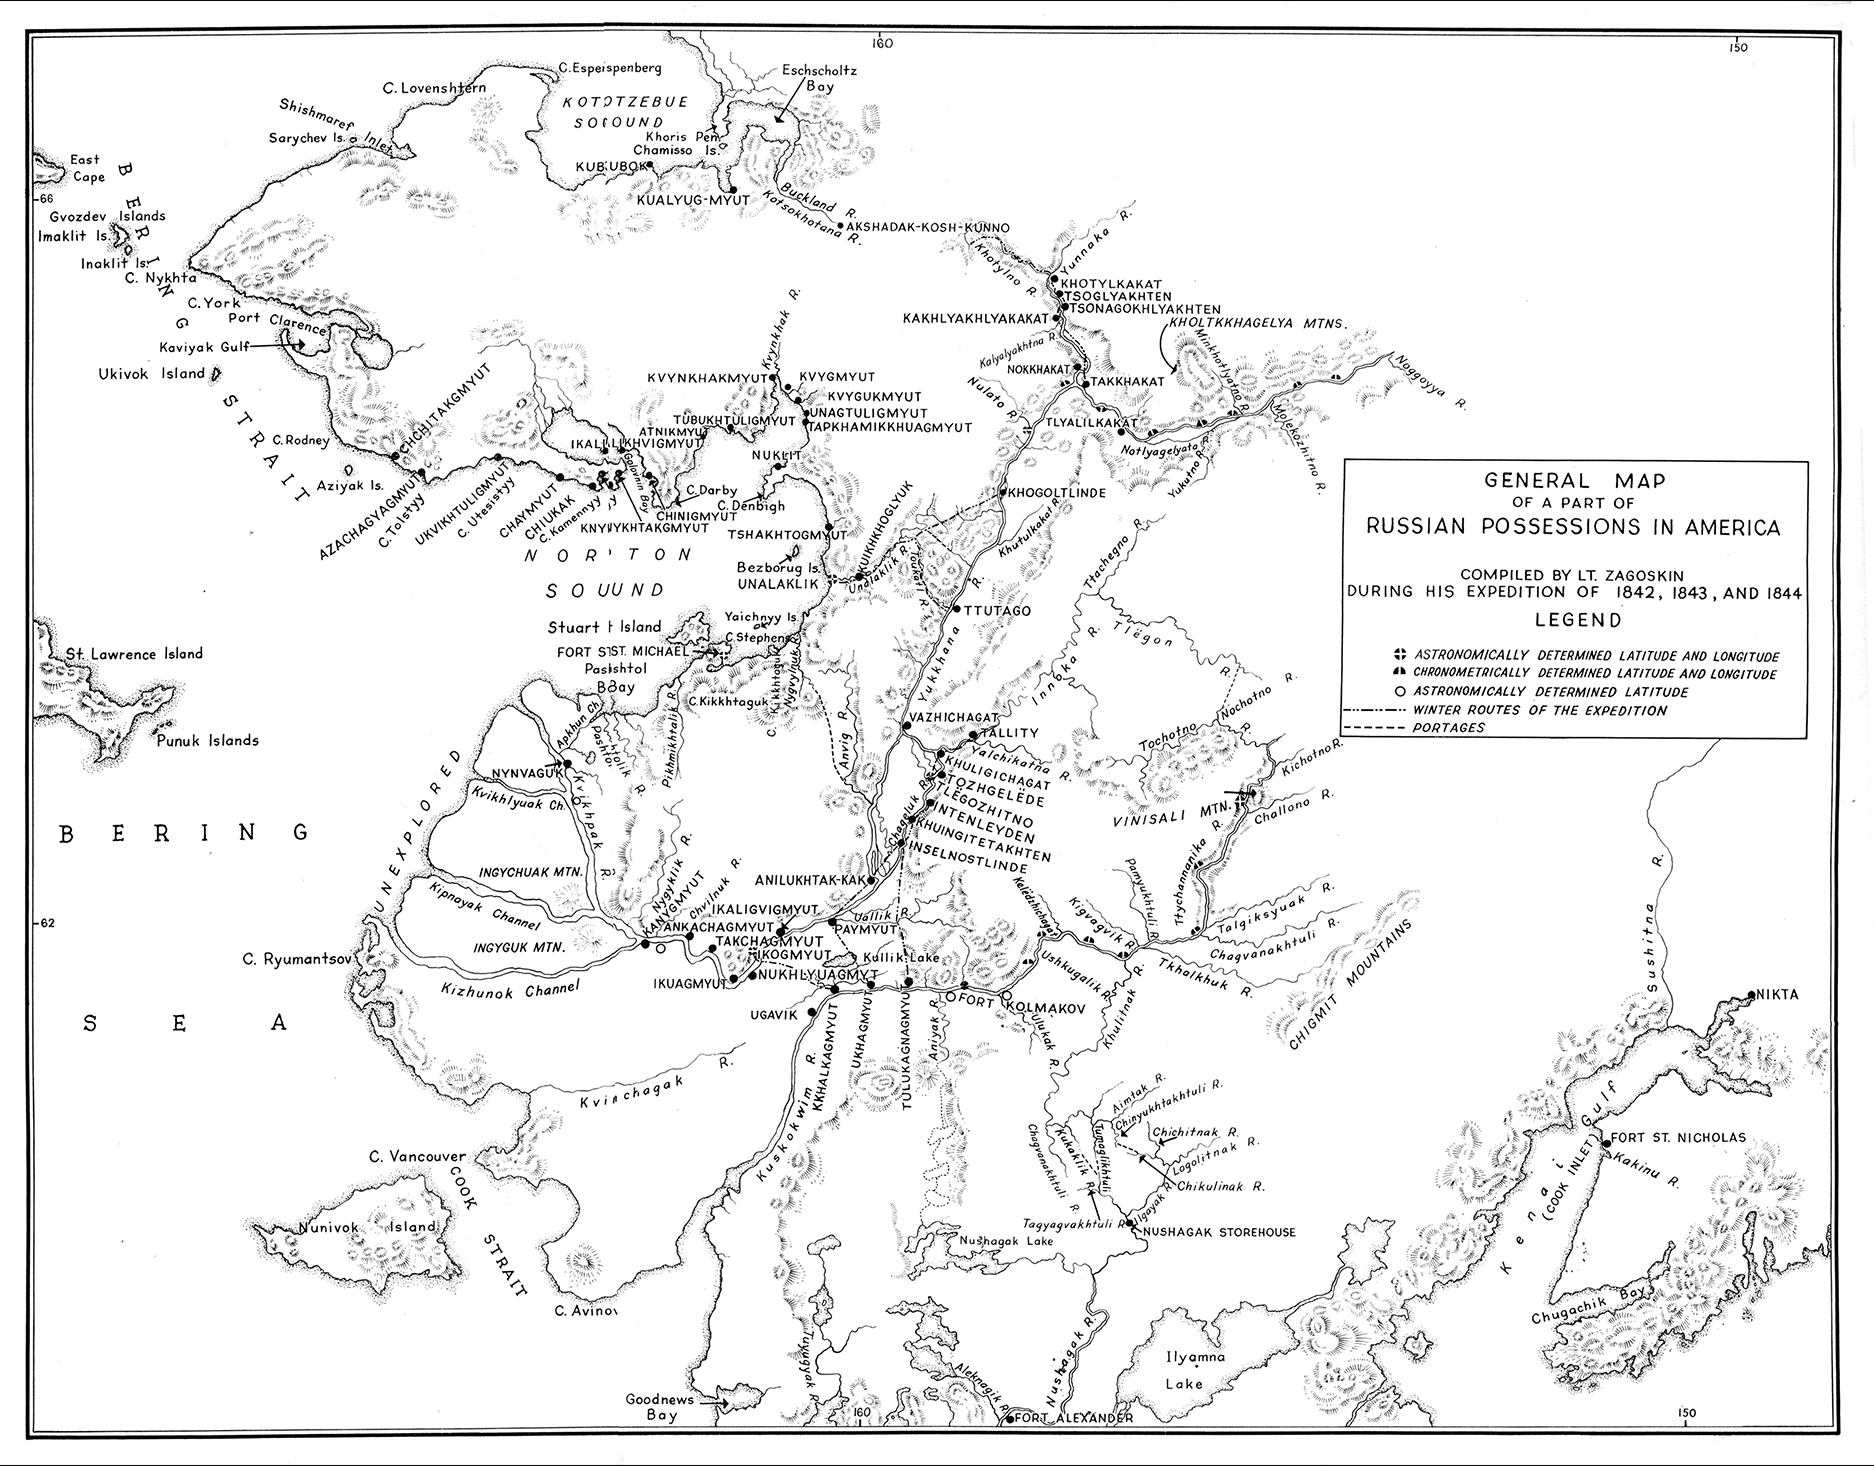
\includegraphics[width=\linewidth,keepaspectratio]{figures/pratt-fig2}
%                    \captionof{figure}{``General Map of a Part of Russian Possessions in America” (Zagoskin 1967 [facing p. 358])}
%         \label{pratt-fig2}
%         \end{minipage}
%    \end{sideways}
%    \end{center}
    
    \begin{figure}[!h]
    \centering
    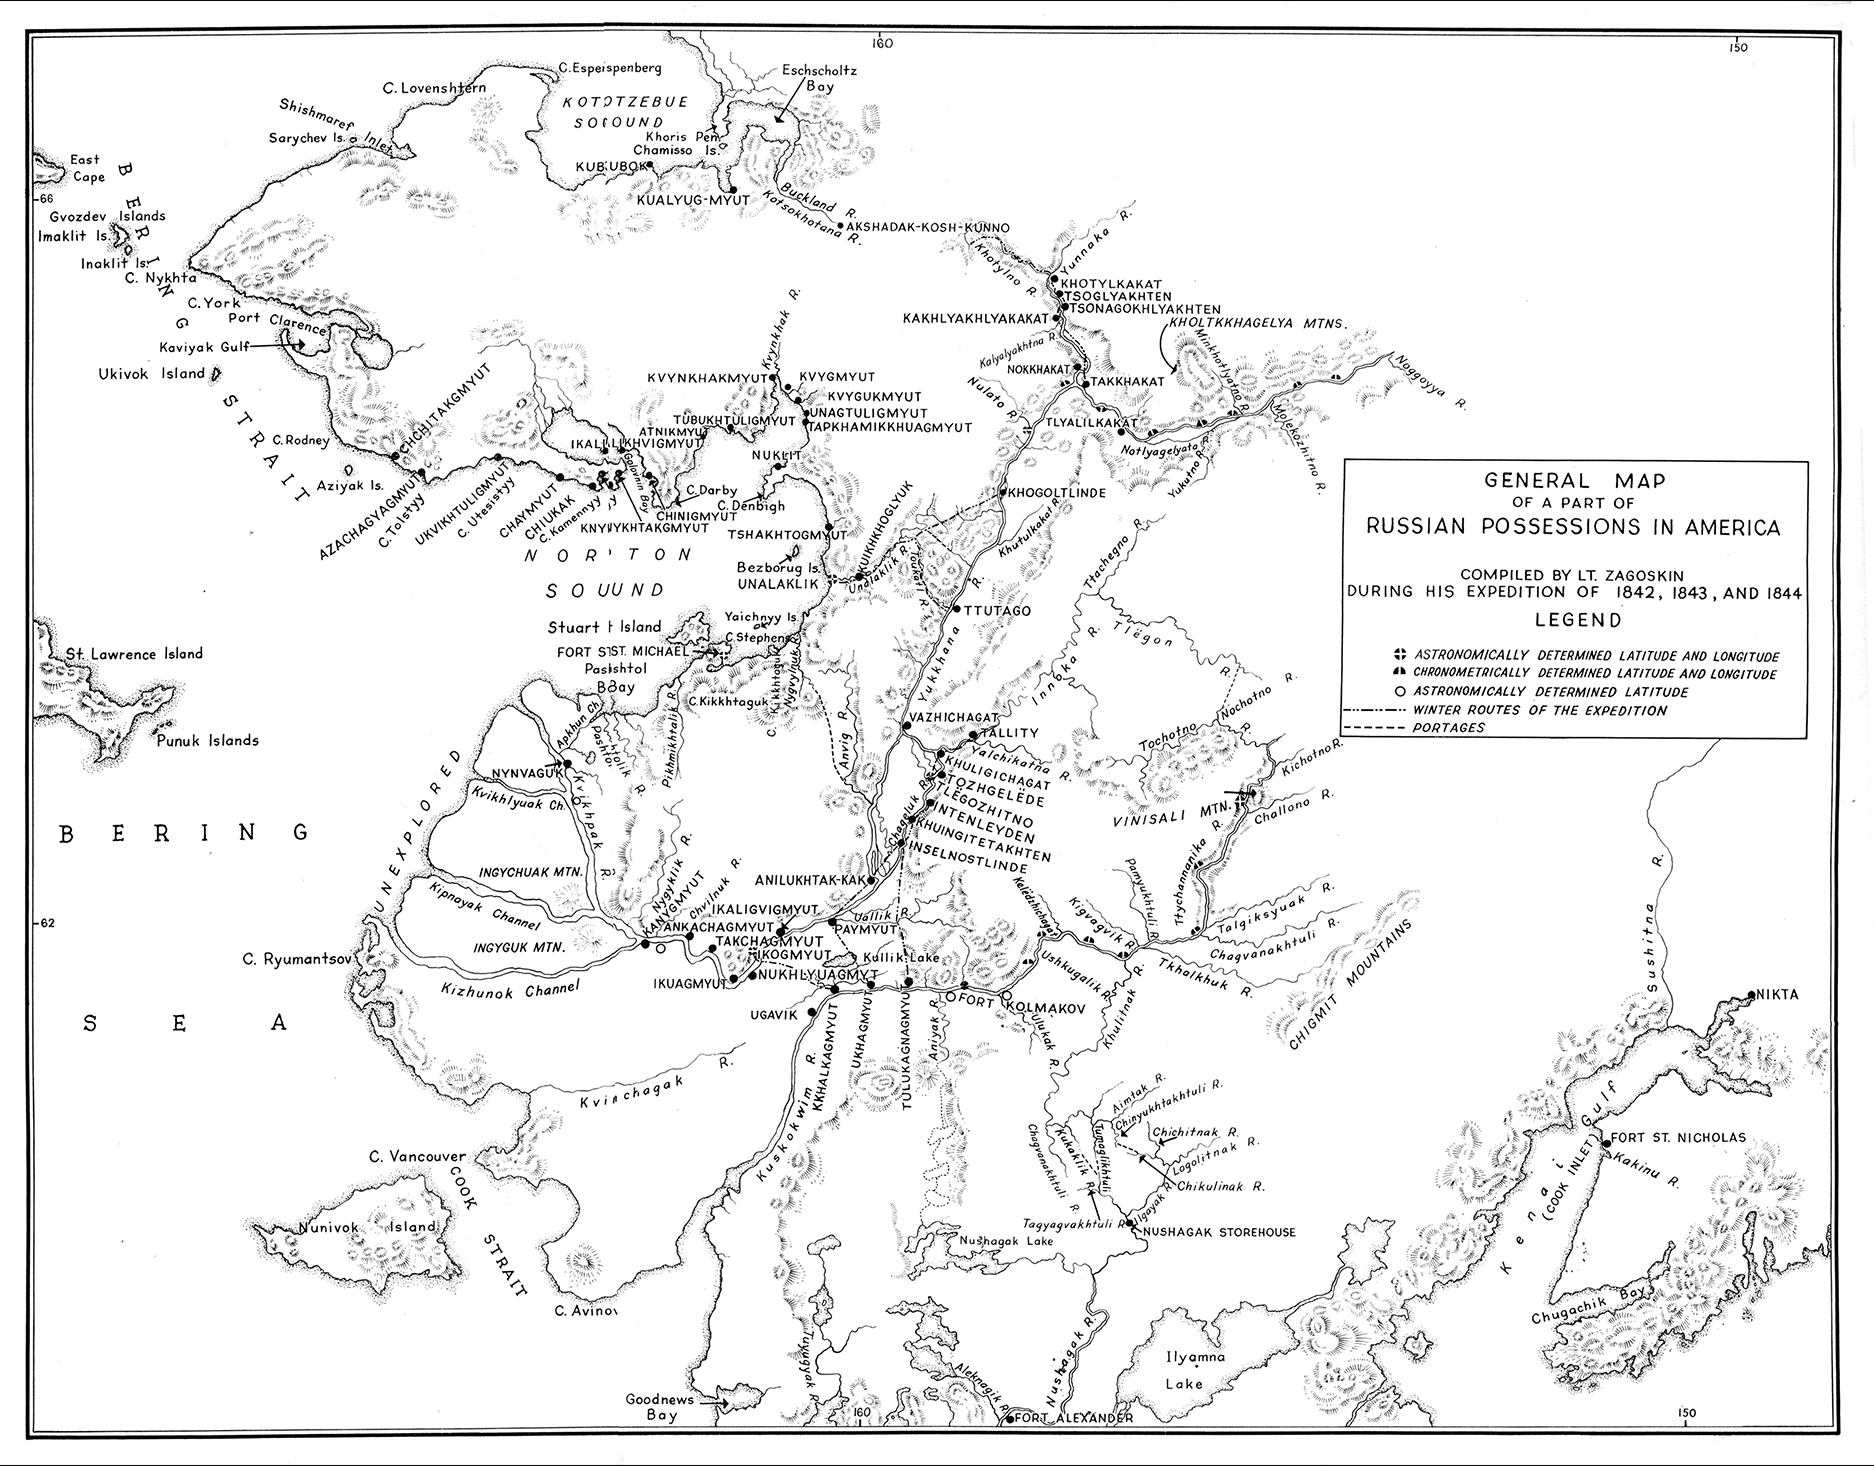
\includegraphics[width=\textwidth]{figures/pratt-fig2}
    \caption{``General Map of a Part of Russian Possessions in America” (Zagoskin 1967 [facing p. 358])}
    \label{pratt-fig2}
\end{figure}

\section*{Sociopolitical Setting}
The Zagoskin expedition was part of an effort begun in about 1818 by the Russian government and the Russian-American trading company to increase knowledge about the geography, resource wealth, and inhabitants of the Bering Sea coast and adjacent interior areas of “Russian America” [Alaska]. Because this region had not previously attracted serious attention from any foreign government the lifeways and traditions of its indigenous residents were intact, despite the presence of Euroamerican trade goods. Trade was, in fact, the main impetus for the expedition (see Arndt 1996: 52-54). A central expectation imposed on Zagoskin was to “find out by what routes furs were being exported from the interior of Alaska for [native] trade with the Chukchi [of Siberia] (Chernenko et al. 1956: 15). The ultimate Russian objective was to intercept furs that otherwise would be lost to established systems of aboriginal trade, such as that which flowed between the middle Yukon River and Norton Sound via the Kaltag Portage (e.g., see Pratt 2012). The collection of detailed information about Alaska Native peoples, their ways of life, and their knowledge of local and regional geography was key to this effort. Whether by accident or design, Zagoskin proved to be a good man for the task.

In both Eskimo and Athabascan populations of the region, the largest cohesive social unit of the Native peoples Zagoskin’s expedition encountered is best described as a “local group”: a somewhat fluid organization of one or more extended families that lacked formalized leadership positions and was centered around the same winter village. Each local group was economically self-sufficient. Its members followed a subsistence lifestyle that, based mainly on resource availability, involved moving between two to five different residence localities over the course of the year. The most populous locales were winter villages, which usually were occupied by two or more extended families for about six months at a time and ranged in population from about 25-100 residents. Historical accounts indicate some winter villages were substantially larger, but they were not common. Thus, in the normal routine of its travels the Zagoskin expedition came into contact with a wide array of small, autonomous Native groups whose relations with other nearby groups—as with their motivations relative to the Russians—could be highly variable. The sociopolitical landscape was complicated and potentially dangerous, thereby requiring careful and deliberate navigation by outsiders.

\section*{Data Collection Challenges on the Zagoskin Expedition}
Communication across language barriers is a critical and often overlooked factor to consider when evaluating ethnographic data about Native populations collected in any colonial setting. This is especially true when that process depended on interpreters, which was virtually always the case relative to nineteenth century Euroamerican explorations in Alaska’s Yukon and Kuskokwim River drainages (e.g., Pratt 2013: 23-25). Even Euroamericans who were comparatively skilled linguistically would have had difficulty communicating with Native groups in this region, as it was home to a number of distinct languages, most comprised of multiple dialects and sub-dialects. But Zagoskin is the only early explorer of the region who consciously alerted future readers of his account to linguistic constraints that affected the completeness and quality of the data he collected from and about Alaska Native peoples. Later visitors to the region (e.g., Edward W. Nelson [1899]) undoubtedly encountered similar problems but their works are generally accepted as historically valid without consideration of potential difficulties in cross-cultural communication—probably due in part to their lack of discussion of such issues. Another unique quality of Zagoskin’s work compared to those of other explorers of the region is that data he obtained directly from Alaska Natives were subjected to critical scrutiny and collected in accordance with a fairly strict methodology. Part of his approach was explained as follows:

\begin{quote}
    I have in general refrained from including information about places unknown to me, places which I could not check by personal observation, unless there was agreement in statements of several natives and an explanatory translation by an interpreter (Zagoskin 1967: 272).
\end{quote}

Zagoskin was in the region for just over two years in the early 1840s, during which time he made eleven separate trips (Pratt 1984: 120 [note 13])\footnote{Zagoskin arrived at St. Michael [Mikhailovskii Redoubt] on 10 July 1842 and departed from the same place for his return to Russia on 5 August 1844.  Chernenko ([1956] 1967: 19) presents a quote from Zagoskin’s diary that could be misread to suggest his tenure in Russian America was less than two years (i.e., “1 year, 6 months, and 16 days”), but it actually refers to the duration of time during which Zagoskin’s expedition was continuously away from St. Michael.} and used the services of at least eight different interpreters: i.e., five Russian Creoles\footnote{In Zagoskin’s usage, ‘Russian Creoles’ were “Those born in Russian America, sons and daughters of Russian fathers and [Alaska] native mothers” (Zagoskin 1967: 330). In the broader history of Russian America, however, the designation “creole” is more complicated (see Black 1990; 2004: 209-220). } and three Athabascan Indians (Pratt 1984: 135-137).  Two of the Athabascan interpreters were from the Koyukuk River area, and the other from the Yukon-Innoko River area. Of the Creole interpreters, two were from unspecified areas of Alaska; the others were from, respectively, Kodiak Island, Cook Inlet, and the Russian colony at Fort Ross, California.\footnote{“Stepanov,” the interpreter from Cook Inlet (Zagoskin 1967: 263, 345), was especially skilled and trusted by Zagoskin (1967:271-272; see also De Laguna 1947: 30). The interpreter from Kodiak Island was Nikifor Talizhuk, and the interpreter from Fort Ross was Pavel Agliaiuk (see Arndt 2015: 10-11). }

Zagoskin relied heavily on Russian post managers Andre Glazunov and Semen Lukin (both Creoles) for data about Yup’ik Eskimos (Zagoskin 1967: 143, 291-292 [note 41]; see also Oswalt 1990: 61). In fact, if his expedition ever specifically employed an Eskimo interpreter it is not clearly indicated in his journal.  But Zagoskin probably received some degree of linguistic aid from Yup’ik Eskimos of Unalakleet who guided him partway up the Unalakleet River (Zagoskin 1967: 133-135; see also Pratt 2012: 101-103); and from a Yup’ik woman [“Kuropatka”] who traveled with the expedition during a three-week trip between Russian Mission [“Ikogmyut”] and Nulato (Zagoskin 1967: 185-194). During the return leg of the latter trip he was also accompanied for a short period by Yup’ik residents of Paimiut (Zagoskin 1967: 194).

The most fundamental problem Zagoskin faced was simply communicating with his expedition—which he said was usually a composite of several Creoles, a few Eskimos and/or Athabascans, and maybe a fellow Russian or a Siberian Native [e.g., Nikitin, the “Tungus” (Zagoskin 1967: 103)].  Conversations with expedition members were generally conducted using a mixture of Russian, Athabascan and Eskimo, one consequence being that the interpreters “often failed to understand the gist of the questions put to them” (Zagoskin 1967: 167, 231).  This limited the information that could be transmitted during contacts with the region’s Native peoples, as indicated in the following statement.

\begin{quote}
    ...to avoid future criticism I feel that it is my duty to explain that all the information I collected here from the Tlegon-khotana [upper Innoko] Natives, as well as from those I met later on, came to me through the following system: every answer to my questions was given to Vtornik [a Koyukuk River Athabascan], who passed it on to Tatlek [another Koyukuk River Athabascan], who told it to the Creole interpreter from our California colony [Nikifor Talizhuk], who told it to me.  Thus, even a perfectly accurate piece of information could be distorted through the oral transfer between interpreters who barely understood each other (Zagoskin 1967: 168).

\end{quote}

Linguistic constraints explain Zagoskin’s reliance on material culture differences as his chief means for identifying and demarcating different Native groups during his expedition (e.g., Zagoskin 1967: 209). This is implied by a comment about his travels in the Koyukuk [“Yunnaka”] River area.

\begin{quote}
The difficulty of communicating through pantomime, and through three interpreters who often could not understand each other, often resulted in our limiting ourselves principally to questions about visible objects (Zagoskin 1967: 153, 295-296 [note 66]).
\end{quote}

\noindent
Zagoskin also noted the impact of language problems on his collection of Native places names.

\begin{quote}
    Our [Dene/Athabascan] guide…had an insufficient command of the [Eskimo] language spoken about us, and for this reason we were often unable to get satisfactory information from him, especially where renditions of place names was concerned (Zagoskin 1967: 232-233).

\end{quote}

\noindent
And also:

\begin{quote}
When we explored upstream [from Nulato] on the Yukon, we went through places where the Tlëgon-khotana people come down to the river, but as we did not have a proper interpreter we could not learn details about the crossing or the name of the river by which they cross (Zagoskin 1967: 300 [note 94]).
\end{quote}

After he had lived in both St. Michael and Nulato for some time, Zagoskin (1967:242) could somewhat understand the language of the former’s Eskimo and the latter’s Athabascan residents, and make himself understood to them (with some difficulty) “in a mixture of dialects.” Interestingly, he suggested that as his own Native language skills \textit{increased} his ability to record vocabulary terms from some groups \textit{decreased}---because his questions began to be answered almost exclusively in the dialects he understood (Zagoskin 1967: 242-243).

The expedition’s dependence on interpreters also forced Zagoskin to deal with the unwillingness of some interpreters to accompany his party into the homelands of groups with which they were unfamiliar or in areas they did not feel safe. One such instance involved the Koyukon Athabascan Tatlek’s reluctance to guide the party beyond the Koyukuk River mouth. Residents of that area warned Tatlek of potential danger in guiding Russians further up the Koyukuk, due to “the unfriendliness of the [Malemiut] and their antagonism towards [the Russians]” (Zagoskin 1967: 150). Zagoskin interpreted this warning as an obvious attempt by one group of traders to protect an avenue of their trade from another. Tatlek was uneasy, however, and only agreed to continue after being threatened with unpleasant consequences that would follow if he chose to abandon the party.

There were also occasions when Zagoskin felt the employment of guides and interpreters had negative effects on his meetings with Native peoples. He noted that when his party was not accompanied by guides or interpreters some groups “manifested a freer and friendlier attitude” and were “more communicative with words and signs”; conversely, he suggested some people’s timidity toward or reluctance to engage with his party “could be ascribed to the influence or attitudes of the guides, who always behave as though they had some sort of guardianship over us” (Zagoskin 1967: 176).

As the preceding comments suggest, Zagoskin’s journal contains numerous comments that describe difficulties in communication between his party and the local peoples with whom it came into contact. Nevertheless, he compiled a rich and remarkably accurate body of data about Native populations. His account is often the only and/or most important source of data available on some aspects of the region’s Native history (e.g., see Snow 1981: 605). Zagoskin’s conscientious documentation of place names (VanStone 1967b:xiii; see also Pratt 2012: 101-105) is a case in point.\footnote{Since the English translation of his journal (Zagoskin 1967) does not include an index, however, finding and extracting the place names data contained therein is a tedious task.} He was intent on collecting the Native names of settlements, hydrographic and topographic features encountered throughout the course of his expedition—and equally averse to applying Russian or honorific names to the landscapes through which he traveled. The latter practice was not followed nearly as rigidly by later explorers in the region. It is also noteworthy that the accounts of some individuals who arrived in the region after Zagoskin, spent more time there, and traveled extensively in connection with their duties (e.g., Iakov Netsvetov [1984]) suggest they devoted considerably less effort to documenting Native place names.

But Zagoskin did more than simply record such names—he also provided important contextual information for many of them. Three relevant examples follow. The first two apply to what is today known as the Innoko River (see Figure~\ref{pratt-fig3}).

\begin{quote}
    A little below [the settlement of Ttality] the river Ttachegno, flowing from the north, joins the Tlёgon. It is from the upper waters of the Ttachegno that the natives cross over to the Yukutno, and on it to the Yuna, or upper Yukon. After the junction of the Tlёgon and the Ttachegno, the river receives the name of Shiltonotno from the natives living in its upper reaches, and Innoka from the people living downstream. In general the direction of the channel is towards the southwest until it joins the Tstseyaka Slough, which flows from the Yukon. From this point…the river changes its name again and is called the Ittege by one tribe and Chagelyuk by the other (Zagoskin 1967: 237).
\end{quote}



\noindent
Here’s another example:

\begin{quote}
    It was 10 miles through woods and often over tundra to Khuligichagat village from the point we had determined, in the general direction of northwest 10°. Sometimes we traveled on the river, sometimes along its right bank. There is a small settlement called Tozhgelёde on the left bank of the Ittege 7 miles before one reaches Khuligichagat. The summer camp of this settlement is situated opposite one of the mouths of a channel which flows from the Yukon into the Ittege and which is called Tstseyaka by the natives. Along the trail we met five sleds and natives from the Iltenleyden settlement who were returning from the coast. They told us they had exchanged their furs at Kikkhtaguk [Klikitarik] village for sealskin and deerhide (Zagoskin 1967: 235).
\end{quote}

\noindent
And finally:

\begin{quote}
    The Talgiksyuak flows out of a small lake. Its width at high water is from 30 to 50 sazhens,\footnote{A \textit{sazhen} is a measure of length equal to 2.1 meters. } in the fall only half of this. Otter are caught here in great numbers, and the fish as they come upstream—whitefish, muksun whitefish, and imagnat [blackfish]. The winter camp of Chinik is situated at its mouth; there are more than 10 camps of the Ikogmyut and Ikaligvigmyut along the river (Zagoskin 1967: 274).
\end{quote}

Linguistic applications notwithstanding, critical analysis of this associated place names information can help researchers to: (a) determine the locations of many of the named places on modern topographic maps; (b) reconstruct Native subsistence and land use patterns; and (c) delineate certain ethnic group boundaries extant at the time of Zagoskin’s expedition. With respect to the last, Zagoskin recognized (1967:298 [note 76], 299 [note 89]) that different groups often had different names for the same river, place or feature (Table~\ref{pratt-tab1}; see also Figure~\ref{pratt-fig4}). When such dual names were recorded he gave precedence to “the local names as a clearer indication of the location of different tribes” living in the area (Zagoskin 1967: 295 [note 65]).


\begin{table}
	\centering
	\small
	\label{pratt-tab1}
	\caption{Selected Athabascan and Eskimo Place Names Reported by Zagoskin, with Known Modern Equivalents.}
	\begin{tabular}{ L{1.5cm} L{4cm} L{3cm} L{3cm} }
\toprule
\textbf{Feature Type}&\textbf{Athabascan~Name}&\textbf{Eskimo~Name}&\textbf{Modern~Name}\\
\midrule
Site&Inselnostlende&Katykhkatmyut&\\
Site&Khuingitetakhten&&\\
Site&Iltenleyden&Unagun-chagelyugmyut&Shageluk\\
Site&Khuligichagat&&Holikachuk\\
Site&Vazhichagat, Makaslat&&\\
Site&Ttality, Totaskholëden&&Dementi\\
Site&&Anilukhtakpak&Gost Creek \\
Site&&Paymyut&Old Paimiut\\
River& \makecell[tl]{Tlëgon [upper] \\ Innoka, Shiltonotno [middle]\\ Ittege [lower] }
          &Chagelyuk&Innoko River\\
River&Yalchikatna&Tachaychagat&Iditarod River\\
River&Tstseyaka [upper]&&Thompson Slough, Holikachuk Slough\\
River&Tstseyaka&&Shageluk Slough\\
River&&Uallik&Paimiut Slough\\
River&\makecell[tl]{Yuna\\Yukkhana}&Kvikhpak&Yukon River\\
River&\makecell[tl]{Ttykini\\Ttychannanika}&Kuskokwim&\makecell[tl]{Kuskokwim River\\Upper Kuskokwim}\\
River&Khottylno&Kvikhchagpak&Crooked Creek\\
River&Kholitna, Khulitnak&&Holitna River\\
River&Khochalitno&Chagvanakhtuli&Swift River\\
River&Talgatno&Talgiksyuak&Tatlawiksuk River\\
		
\bottomrule		
		
	\end{tabular}
\end{table}


Detailed observations by Zagoskin about local environmental landscapes through which his party passed sometimes provide deeper contexts for certain Native place names. His remarks about the “Innoka” River are a case in point.

\begin{quote}
    The extraordinary width of the [Yukon] river is certainly explained by the speed and the enormous quantity of water which pours into it during the spring floods from all its tributaries. As all these waters cannot be contained in the channel, they wash away and cut into the banks, creating the innumerable islands which we found between Nulato and Vazhichagat. Below this point the Yukon displays another surprising peculiarity: when the Tstseyaka and other sloughs split off from it, more than half of its waters flow into the Innoka, creating various low but sizeable islands which are dotted with lakes stocked with fish (Zagoskin 1967: 195).
\end{quote}
\noindent
This description expands Jette’s (n.d.:110-111) later explanation of the Innoko (i.e., Lurno [“fish river”]) place name, which was summarized by the following statement: “The Innoko River is remarkable for the abundance of fish in its waters, hence its name.”

\section*{Concluding Remarks}
The importance of Zagoskin’s work is clearly recognized by numerous scholars who have used and become familiar with the journal of his expedition (e.g., Arndt 1996: 59-65; Bockstoce 2009: 194-196; Brooks 1953: 232-234; De Laguna 1947: 29 [note 19], 31; Orth 1967: 43-44; Oswalt 1967: 233; VanStone 1967b; 1979b:78). I count myself among that group, having likely used the report of Zagoskin’s expedition more extensively than any other scholar—both for personal research (e.g., Pratt 1984, 2012) and in my official capacity documenting Alaska Native cultural sites (see Pratt 2009)—and consistently finding his data to be highly reliable. Unfortunately, Zagoskin was harshly criticized by William H. Dall (1877:22; cf. De Laguna 1947: 29 [note 19], 31; 2000: 33-34), whose opinion on the subject is at best ironic given the dubious accuracy of some of his own work (see Arndt 1996: 177; Petroff 1884: 161; Ray 1975: 133-134; VanStone and Goddard 1981: 561). Youthful arrogance was likely a factor, but Dall’s criticism of Zagoskin may also have been influenced by the general disdain he seemed to hold for Russians in Alaska (e.g., see De Laguna 2000: 187-188). Less understandable is the fact that Zagoskin has also been maligned by several prominent scholars who arguably did not make serious efforts to utilize his account (i.e., Black 1984: 30 [see also Netsvetov 1984:xx; cf. Oswalt 1990: 59-61]; Burch 1984: 9).\footnote{In his last major publication, Burch (2012) put considerable stock in Zagoskin’s observations about caribou in western Alaska. True to his penchant for scholarly honesty, when questioned about his 1984 criticism of Zagoskin versus his new reliance on the explorer’s account Burch (personal communication, 2/10/2010) explained that his original, negative impression was based on comments about Zagoskin’s work received from a respected colleague.} One indirect goal of this paper is to objectively challenge and counteract these negative assessments of Zagoskin’s report. Another is to make the point that problems involving cross-cultural communication—although rarely mentioned—arguably posed greater challenges to the success of early Euroamerican explorers of the Yukon-Kuskokwim region than did the physical hardships they encountered.

This brief summary of Zagoskin’s work provides a foundation for critically reviewing the Native place names data he collected. Minimally, any such review should include at least three tasks.

\begin{enumerate}

    \item  Searching the writings of other early authors and more recent sources relevant to the geographical area of focus to determine if some of the same places for which Zagoskin recorded names are represented in their works.
    \item Critically comparing locational information provided by Zagoskin about specific named places against modern topographical maps in an effort to accurately correlate the names with discrete places on the physical landscape.\footnote{Henry N. Michael, editor of the 1967 English translation of Zagoskin’s journal, did a remarkably good job in his own efforts to make such correlations—particularly considering his lack of personal knowledge of the regions of Alaska visited by Zagoskin’s expedition. Another benefit of this comparative task is that it sometimes reveals significant errors on published United States Geological Survey (USGS) maps. The present case yielded several examples of such errors (e.g., refer to the place names “Kakyglët” and “Kukaklik Lake” in the Appendix). Finally, in 2010 and 2011 Russian explorer Mikhail Malakhov organized and led expeditions to Alaska that followed routes taken by nineteenth century Russian explorers along the Yukon-Kuskokwim Portage and an overland trail between the Kuskokwim and Nushagak Rivers. The expedition’s findings were helpful in resolving several problematic correlations with place names reported by Zagoskin.}
    \item Undertaking the necessary linguistic research to correct (consistent with accepted Alaska Native language orthographies), or at least improve, place name spellings Zagoskin reported.
\end{enumerate}

Although none could be done in a truly comprehensive fashion, each of the tasks just described was essential to producing the Appendix to this paper. It lists place names found in Zagoskin’s comparatively short accounts of his trips between the Yukon River village of “Ikogmyut” (Russian Mission), the Innoko River and upper Kuskokwim River from November 1843 to June 1844 (see also Figures~\ref{pratt-fig5} and \ref{pratt-fig6} in the Appendix). The 45 journal pages that describe those trips (i.e., Zagoskin 1967: 199-208, 231-242, 249-274) reference 145 named places: most are identified with Native place names, reflecting multiple languages (e.g., Central Yup’ik, Deg Xinag, Holikachuk, Koyukon, Upper Kuskokwim, Dena’ina). Significantly, my findings suggest that about half of these place names do not appear in Donald Orth’s (1967) encyclopedic Dictionary of Alaska Place Names. This underscores the great potential Zagoskin’s 300+ page journal holds for increasing the current inventory of Native place names in Alaska.


\section*{Acknowledgements}
I wish to thank Jim Kari for his generous help and sharing of data associated with my efforts to correlate and correct spellings of certain Native place names recorded by Zagoskin; Robert Drozda, Matt O’Leary and Mikhail Malakhov for assistance related to the Appendix; Dale Slaughter for his work on the maps contained herein; Katherine Arndt for providing me with biographical information about the namesake of “Slatin post”; an anonymous reviewer for helpful comments on a draft of the paper; and Gary Holton for inviting me to contribute to this volume.


\refheading
\begin{hang}

Anvil, Oscar. 1988. Tape recorded oral history account. Ted Krieg, interviewer; Mary Gregory, interpreter. Bethel, Alaska; 6 July. Tapes 88CAL053 and 88CAL054. Bureau of Indian Affairs, ANCSA Office, Anchorage.

Arndt, Katherine L. 1996. \textit{Dynamics of the Fur Trade on the Middle Yukon River, Alaska, 1839 to 1868}. Ph.D. dissertation, Department of Anthropology, University of Alaska Fairbanks.

Arndt, Katherine L. 2015. Transplanted to a Northern Clime: Californian Wives and Children in Russian Alaska. \textit{Alaska Journal of Anthropology} 13(2). 1-20.

Arundale, Wendy H. 1983. \textit{Doyon Historic Sites Project Report: Innoko Area}. Doyon, Limited, Fairbanks. (Copy on file at Bureau of Indian Affairs, ANCSA Office, Anchorage.)

Black, Lydia T. 1984. The Yup’ik of Western Alaska and Russian Impact. \textit{Etudes/Inuit/Studies} 8 (Supplementary Issue). 21-43.

Black, Lydia T. 1990. Creoles in Russian America. \textit{Pacifica} 2(2). 142-155.

Black, Lydia T. 2004.	\textit{Russians in Alaska, 1732-1867}. University of Alaska Press, Fairbanks.

Bockstoce, John R. 2009. \textit{Furs and Frontiers in the Far North: The Contest among Native and Foreign Nations for the Bering Strait Fur Trade}. Yale University Press, New  Haven and London.

Brooks, Alfred H. 1953. \textit{Blazing Alaska’s Trails}. University of Alaska Press, Fairbanks.

Burch, Ernest S., Jr. 1984. The Central Yup’ik Eskimos: An Introduction. \textit{Etudes/Inuit/Studies} 8 (Supplementary Issue). 1-19.

Burch, Ernest S., Jr. 2012. \textit{Caribou Herds of Northwest Alaska, 1850-2000}. Edited by Igor Krupnik \& Jim Dau. University of Alaska Press, Fairbanks.

Chernenko, Mikhail Borisovich. 1967[1956]. Lavrentiy Alekseyevich Zagoskin: An Account of His Life and Works.  In Henry N. Michael (ed.), \textit{Lieutenant Zagoskin’s Travels in Russian America, 1842-1844}, 3--34. Translated by Penelope Rainey.  University of Toronto Press, Toronto.

Chernenko, M.B., G.A. Agranat \& Y.E. Blomkvist. 1956. \textit{The Travels and Explorations of Lieutenant Lavrentiy Zagoskin in Russian America, 1842-1844}. State Publishing House of Geographic Literature, Moscow.

Dall, William H. 1877. \textit{Tribes of the Extreme Northwest}. Contributions to North American Ethnology, Vol. 1. Government Printing Office, Washington, DC.

De Laguna, Frederica. 1947. \textit{The Prehistory of Northern North America as Seen from the Yukon}. Memoirs of the Society for American Archaeology, Number 3. Menasha, WI.

De Laguna, Frederica. 2000. \textit{Travels among the Dena: Exploring Alaska’s Yukon Valley}. University of Washington Press, Seattle and London.

Ellanna, Linda J. \& Andrew Balluta. 1992. \textit{Nuvendaltin Quht’ana: The People of Nondalton}. Smithsonian Institution Press, Washington, DC and London.

Fienup-Riordan, Ann (ed.). 1988. \textit{The Yup’ik Eskimos: As Described in the Travel Journals and Ethnographic Accounts of John and Edith Kilbuck, 1885-1900}. Edited, with an Introduction by Ann Fienup-Riordan. Limestone Press, Kingston, ON.

Fienup-Riordan, Ann (ed.). 2014. \textit{Nunamta Ellamta-llu Ayuqucia (What Our Land and World Are Like): Lower Yukon History and Oral Traditions}. Translated and Transcribed by Alice Rearden; edited by Ann Fienup-Riordan. Calista Elders Council (Anchorage) and Alaska Native Language Center, University of Alaska Fairbanks.

Grinev, Andrei. 2009. \textit{Kto est’ kto v istorii Russkoi Ameriki [Who is who in the history of Russian America]}. Academia, Moskva.

Hosley, Edward H. 1981. Kolchan. In June Helm (ed.), \textit{Handbook of North American Indians, vol. 6: Subarctic}, 618-622. Washingon, DC: Smithsonian Institution Press.

Ignati, Evan. 1994. Tape recorded oral history account. Robert Drozda, interviewer. Fairbanks, Alaska; 28 October. Tape 94HOL001.RD. Copy on file, Bureau of Indian Affairs, ANCSA Office, Anchorage.

Jette, Jules. n.d.	On the Geographical Names of the Ten’a. “Jottings of a Missionary,” unpublished manuscripts, Alaska Mission Collection, M/F 96, roll 34, Rasmuson Library Archives, University of Alaska Fairbanks.

Kari, James (ed.). 2015. \textit{Upper Kuskokwim Athabascan Place Names Lists}. Unpublished manuscript, Alaska Native Language Center, University of Alaska Fairbanks.

Kari, James \& James A. Fall. 2003. \textit{Shem Pete’s Alaska: The Territory of the Upper Cook Inlet Dena’ina} (2nd edition). University of Alaska Press, Fairbanks.

Kari, Priscilla Russell. 1983. \textit{Land Use and Economy of Lime Village}. Technical Paper No. 80, Alaska Department of Fish and Game, Division of Subsistence, Juneau.

Kari, Priscilla Russell. 1985. \textit{Wild Resource Use and Economy of Stony River Village}. Technical Paper No. 108, Alaska Department of Fish and Game, Division of Subsistence, Juneau.

Malakhov, Mikhail. 2011a.	Kuskokwim-Yukon-63K-MalakhovRoute (map). \url{https://cloud.mail.ru/public/9nV9/okP5Zt7oK}

Malakhov, Mikhail. 2011b	Nushagak-Kuskokwim-250K-MalakhovRoute (map). \url{https://cloud.mail.ru/public/CAm8/z4RByjM2r}


Mikhail, Gusty. 1980. Kuskokwim River Place Names (interview). Jim Kari, interviewer and transcriber (with Yup’ik names transcribed by Steve Jacobson). Stony River, Alaska; 23 November. Tape Ik14. Fairbanks: Alaska Native Language Archive.

Nelson, Edward W. 1899.	\textit{The Eskimo about Bering Strait}. Bureau of American Ethnology, 18th Annual Report, part 1, 1896-97. Government Printing Office, Washington, DC.

Netsvetov, Iakov. 1984. \textit{The Journals of Iakov Netsvetov: The Yukon Years, 1845-1863}. Translated, with an Introduction and Supplementary Material by Lydia T. Black. Edited by Richard A. Pierce. Limestone Press, Kingston, ON.

Orth, Donald J. 1967. \textit{Dictionary of Alaska Place Names}. Geological Survey Professional Paper 567. Government Printing Office, Washington, DC.

Osgood, Cornelius. 1958.	\textit{Ingalik Social Culture}. Yale University Publications in Anthropology, no. 53. Yale University Press, New Haven, CT.

Oswalt, Wendell H. 1967. \textit{Alaskan Eskimos}. Chandler Publishing Company, San Francisco.

Oswalt, Wendell H. 1980. \textit{Historic Settlements along the Kuskokwim River, Alaska}. Alaska State Library Historical Monograph No. 7, Juneau.

Oswalt, Wendell H. 1990. \textit{Bashful No Longer: An Alaskan Eskimo Ethnohistory, 1778—1988}. University of Oklahoma Press, Norman and London.

Petroff, Ivan. 1884. \textit{Report on the Population, Industries, and Resources of Alaska: Tenth Census of the U.S.A., 1880}. Government Printing Office, Washington, DC.

Phillip, Joshua. 1988. Tape recorded oral history account. Robert Drozda, interviewer; Vernon Chimegalrea, interpreter. Tuluksak, Alaska; 29 June. Tape 88CAL046. Bureau of Indian Affairs, ANCSA Office, Anchorage.

Porter, Robert P. 1893. \textit{Report on the Population and Resources of Alaska at the Eleventh Census: 1890}. Government Printing Office, Washington, DC.

Pratt, Kenneth L. 1984. Yukon-Kuskokwim Eskimos, Western Alaska: Inconsistencies in Group Identification.  M.A. thesis, Department of Anthropology, Western Washington University, Bellingham.

Pratt, Kenneth L. 2012. Reconstructing 19th-Century Eskimo-Athabascan Boundaries in the Unalakleet River Drainage. \textit{Arctic Anthropology} 49(2). 14-112.

Pratt, Kenneth L. 2013. Deconstructing the Aglurmiut Migration: An Analysis of Accounts from the Russian-America Period to the Present. \textit{Alaska Journal of Anthropology} 11(1-2). 17-36.

Pratt, Kenneth L. (ed.). 2009. \textit{Chasing the Dark: Perspectives on Place, History and Alaska Native Land Claims}. Edited by Kenneth L. Pratt. U.S. Department of the Interior, Bureau of Indian Affairs – Alaska Region, ANCSA Office, Anchorage.

Ray, Dorothy Jean. 1975. \textit{The Eskimos of the Bering Strait, 1650-1898}. University of Washington Press, Seattle and London.

Smith, Louis. 1990. Tape recorded oral history account. Mary Ellen Fogarty, interviewer; Marie Meade, interpreter. Goodnews Bay, Alaska; March 9. Tape 90PLA005. Bureau of Indian Affairs, ANCSA Office, Anchorage.

Snow, Jeanne H. 1981. Ingalik. In June Helm (ed.), \textit{Handbook of North American Indians, vol. 6: Subarctic}, 602-617. Washington, DC: Smithsonian Institution Press.

Townsend, Joan B. 1965. \textit{Ethnohistory and Culture Change of the Iliamna Tanaina}. Ph.D. dissertation, Department of Anthropology, University of California Los Angeles. University Microfilms, Inc., Ann Arbor.

United States, Bureau of Indian Affairs (USBIA). 1991a.	Report of Reinvestigation for Old Paimiut, AA-12370 (Doyon, Limited). Written by Ronald J. Kent \& Matthew O’Leary. Bureau of Indian Affairs, ANCSA Office, Anchorage.

United States, Bureau of Indian Affairs (USBIA). 1991b.	Report of Investigation for Khuingitetakhten, AA-12363 (Doyon, Limited). Written by Ronald J. Kent, Thomas J. Turck \& Debra Corbett. Bureau of Indian Affairs, ANCSA Office, Anchorage.


United States, Bureau of Indian Affairs (USBIA). 2008. Supplemental Report for Island Village, AA-12360 (Doyon, Limited). Written by Rita A. Miraglia. Bureau of Indian Affairs, ANCSA Office, Anchorage.

VanStone, James W. 1967a.	\textit{Eskimos of the Nushagak River: An Ethnographic History}. Seattle: University of Washington Press.

VanStone, James W. 1967b.	Introduction.  In Henry N. Michael (ed.), \textit{Lieutenant Zagoskin’s Travels in Russian America, 1842-1844}, xi--xiv. Translated by Penelope Rainey.  University of Toronto Press, Toronto.

VanStone, James W. 1978. \textit{E.W. Nelson’s Notes on the Indians of the Yukon and Innoko Rivers, Alaska}. Edited with an introduction by James W. VanStone. Fieldiana Anthropology, Volume 70. Field Museum of Natural History, Chicago.

VanStone, James W. 1979a.	\textit{Historic Ingalik Settlements along the Yukon, Innoko, and Anvik Rivers, Alaska}. Fieldiana Anthropology, Volume 72. Field Museum of Natural History, Chicago.

VanStone, James W. 1979b.	\textit{Ingalik Contact Ecology: An Ethnohistory of the Lower-Middle Yukon, 1790—1935}. Fieldiana Anthropology, Volume 71. Field Museum of Natural History, Chicago.

VanStone, James W. (ed.). 1988. \textit{Russian Exploration in Southwest Alaska: The Travel Journals of Petr Korsakovskiy (1818) and Ivan Ya. Vasilev (1829)}. Edited with an Introduction by James W. Vanstone; translated by David H. Kraus. University of Alaska Press, Fairbanks.

VanStone, James W. \& Ives Goddard. 1981. Territorial Groups of West-Central Alaska before 1898. \textit{Handbook of North American Indians, vol. 6: Subarctic}. Washington, DC: Smithsonian Institution Press.

Williams, Sinka \& Stanley Nook. 1988. Tape recorded oral history account. Philippa Coiley, interviewer. Lower Kalskag, Alaska; 20 July. Tape 88CAL081. Bureau of Indian Affairs, ANCSA Office, Anchorage.

Wright, Miranda. 1995. The Last Great Indian War (Nulato, 1851). M.A. thesis, Department of Anthropology, University of Alaska Fairbanks.

Zagoskin, Lavrentiy A. 1967. \textit{Lieutenant Zagoskin’s Travels in Russian America, 1842-1844: The First Ethnographic and Geographic Investigations in the Yukon and Kuskokwim Valleys of Alaska}.  Translated by Penelope Rainey; edited by Henry N. Michael.  University of Toronto Press, Toronto.


\end{hang}

\vspace{1cm}
\orcidfooter{Kenneth L. Pratt}{kenneth.pratt@bia.gov}{}



%%%%%%%%%%%%%%% appendix follows %%%%%%%%%%%%%%%%%%%%%%%

\clearpage
\noindent
\textbf{\large Appendix: Place Names} \\


\noindent
This Appendix lists the 145 named places mentioned by Zagoskin in four of his party’s trips, the combined accounts of which cover a total of 45 pages in his journal. Place names are listed in the order they were reported during each trip—with the caveat that each place name is listed only once (on the first occasion of its mention). Thus, a place name mentioned in all four of the trips being considered would only appear below in connection with the first trip.



The place name spellings provided in Zagoskin’s journal are \hl{boldfaced}\todo{bolding is copied from the original word document}, with any translations he reported following in parentheses. Italicized place names denote Native language spellings. When known, the Alaska Native language of origin for a place name is indicated by one of the following abbreviations: CY (Central Yup’ik), DH (Deg Hit’an), D (Dena’ina), H (Holikachuk), K (Koyukon), or UK (Upper Kuskokwim). Time limitations precluded any serious attempt to gather and compile place name translations. The feature type to which a given place name is attached is noted; so are correlations to locales (see Figures~\ref{pratt-fig5} and \ref{pratt-fig6}, hydrographic or topographic features named on modern United States Geological Survey (USGS) maps.



In a number of cases, extra contextual information Zagoskin recorded about places named in his account has been included to give readers a better overall sense of the range of information collected during his Alaska travels. Zagoskin's remarks are often supplemented with related comments by the author.


\vspace{1cm}
\noindent
\textbf{Trip 1: Ikogmyut to Fort Kolmakov [23 November – 6 December 1843]
(Zagoskin 1967: 203-208 [22 place names])}
\vspace{6pt}

\begin{hang}

\textbf{Ikogmyut} [\textit{Iqugmiut} (CY)]: winter village, and site of the Russian post Ikogmyut Odinochka (est. 1835); present-day Russian Mission.



\textbf{Kuskokwim}: watercourse; USGS Kuskokwim River.



\textbf{Fort Kolmakov}: Kolmakovskii Redoubt (est. 1832); located on left (south) bank of Kuskokwim River opposite the mouth of USGS Kolmakov River (see Oswalt 1980: 90 [Map 3]).



\textbf{Paymyut} [\textit{Paimiut} (CY)]: winter village; Old Paimiut, abandoned ca. 1880s. Historically, this was the uppermost Eskimo village on the Yukon River. (Note: the site Zagoskin visited is not USGS Paimiut—which was established in the mid-1930s, is located on the opposite (i.e., right) bank of the Yukon, and is the most recent of five sites in the immediate vicinity that were all known as “Paimiut.”)



\begin{quote}“Paymyut ...is situated on the left bank at the confluence of the Yukon and the Uallik. From this village there is an all-year trail to the Kuskokwim” (Zagoskin 1967: 194). The trail referred to here was the Yukon-Kuskokwim Portage.
\end{quote}



\textbf{Yukon}: watercourse; USGS Yukon River.



\textbf{Kkhalkagmyut} [\textit{Qalqarmiut} (CY)]: winter village; Old Kalskag, abandoned ca. 1915 (Oswalt 1990: 122; see also Oswalt 1980: 71-72). This site is located downriver from present-day Lower Kalskag and is not depicted on USGS maps.



\textbf{Ikaligvigmyut} (“fishy”) [\textit{Iqallugvigmiut} (CY)]: winter village; USGS Dogfish Village.



\textbf{Uallik River} [\textit{Ualiq} (CY)]: watercourse; USGS Paimiut Slough.



\textbf{Pashtol} [\textit{Pastuliq; Pastuliarraq} (CY)]: winter village; USGS Pastolik. A major Yup’ik Eskimo village located near the north mouth of the Yukon River; abandoned ca. 1963.



\textbf{Tashatulit}: mountains; USGS Portage Mountains.



\textbf{Ingytkvyygat} (“mountain stream”): watercourse; location uncertain.



\textbf{Tulukagnagmyut} (“crow”) [\textit{Tulukarnermiut} (CY)]: USGS Crow Village. According to Oswalt (1980:38), “In early historic times this was the farthest inland village along the Kuskokwim of exclusively Yupik-speaking Eskimos.”



\textbf{Ukhagmyut} [\textit{Urr’armiut} (CY)]: winter village; USGS Ohogamiut (on Kuskokwim River).



\textbf{Fort Alexander}: Aleksandrovskii Redoubt (est. 1819), located on Nushagak Bay at the mouth of Nushagak River. Also sometimes called the “Nushagak post” (e.g., Zagoskin 1967: 241).\textbf{ }



\textbf{Nushagak}: winter village; Native village at the mouth of Nushagak River (the same location at which Alexandrovskii Redoubt was established).



\textbf{Nuskagak Lakes}: this term of reference likely applied to all of the lakes in the USGS Wood River Lakes and USGS Tikchik Lakes systems.



\textbf{Nushagak}: lake; USGS Tikchik Lake (VanStone 1988: 95).



\textbf{Aniak River} [\textit{Anyaraq} (CY)]: watercourse; USGS Aniak River.



\textbf{Innoka} [\textit{Eniq, Enigg }(DH) \textit{or Yoonig} (H) (Arundale 1983: 48): watercourse. In Zagoskin’s usage this is the middle section of USGS Innoko River.



\textbf{Kukhlyukhtakpak} (“big waterfall”): a camp of the people of Kvygympaynagmyut located on the left bank of Kuskokwim River just downstream from present-day Chuathbaluk (see Oswalt 1980: 48 [“Kukuktuk”], 90 [Map 3]). Zagoskin (1967:232) also identified the site as the “Kukhlyukhtakpak trail house” when his party overnighted there before embarking on the overland trail from the Kuskokwim to the lower Innoko River.



\textbf{Kvygympaynagmyut} [\textit{Kuigem Paingarmiut} (CY)] (also \textbf{Kvygympayma} [\textit{Kuigem Painga} (CY)]: winter village; located on right (north) bank of Kuskokwim River at mouth of USGS Kolmakov River (opposite “Fort Kolmakov”). Also the site of “Lukin’s Odinochka”—built in 1833, the forerunner of Kolmakovskii Redoubt (e.g., Oswalt 1990: 50-51).



\textbf{Fort St. Michael}: Mikhailovskii Redoubt (est. 1833), located on St. Michael Island in southern Norton Sound, at the site of \textit{Taciq}, a Yup’ik Eskimo winter village.

\end{hang}


\vspace{1cm}
\noindent
\textbf{Trip 2: Fort Kolmakov to the Lower Innoka River and Return to Ikogmyut [10 February – 25 March 1844] (Zagoskin 1967: 231-242 [46 place names])}
\vspace{6pt}

\begin{hang}
\textbf{Ittege} [\textit{Edixi} (DH) [Eter’e (Jetté n.d.:83-84)]: watercourse. In Zagoskin’s usage this is the lower section of USGS Innoko River. (\textit{Edixi} = the ‘upper area’ name for the Shageluk village area [Jim Kari, personal communication, 11/28/2015].)



\textbf{Tachatalyatna}: watercourse (a ‘mountain stream’); location uncertain.



\textbf{Anilukhtakpak} [DH]: winter village; USGS Gost Creek, located on the left bank of USGS Walker Slough near present-day Holy Cross (see VanStone 1979a:61-62).



\begin{quote}“[Anilukhtakpak is] the last settlement of the Ttynay [Dene (Athabascan)] on the Yukon: farther downstream and on all the branches of this river, on the Kuskokwim flats, and along the coast to the Alaska Peninsula the people are of the Kang-yulit [Eskimo] tribe” (Zagoskin 1967: 193).
\end{quote}



\textbf{Kykhtulit} [\textit{Digheloye Chin} (UK)]: mountains; “western piedmont, edge of Alaska Range above treeline” (Kari 2015: 13 [no. 168]). Also referred to as “the Kykhtulit Range” (e.g., Zagoskin 1967: 251-252).



\begin{quote}Kykhtulit was described as the ridge that “divides the basin of the Kuskokwim from the waters of Nushagak” (Zagoskin 1967: 232).
\end{quote}



\textbf{Chuazhutl}: mountain group; location uncertain.



\textbf{Tagasushku}: mountain group; location uncertain.



\textbf{Nantlinde}: mountain group; location uncertain.

\begin{quote}
	“The mountain range which stretches northward from the Tashatulit [Portage Mountains] mass to the left bank of the Ittege can be seen at a distance of 25 to 30 miles from the [Yukon-Kuskokwim Portage] trail. Separate mountain groups are called by the natives Chuazhutl, Tagasushku, and Nantlinde. The Uallik [Paimiut Slough] has its source on the slopes of the first two of these groups” (Zagoskin 1967: 232).
\end{quote}



\textbf{Kullik} (“trousers”) [\textit{Qerrulliik} (CY)]: watercourse [“one of the tributaries of the Uallik” (Zagoskin 1967: 233)]; probably USGS Twelvemile Slough.



\textbf{Kauvak}: camp; location uncertain.



\textbf{Naumgyk}: watercourse [a small river “which falls into one of the tributaries of the Uallik” (Zagoskin 1967: 233)].



\textbf{Inselnostlende} [DH] or \textbf{Katykhkatmyut} [CY]: winter village. As confirmed by BIA ANCSA researchers in 2007, the site location is on the right bank of Innoko River about 20 miles south of Shageluk. The site corresponds with Osgood’s (1958:30) “Island-Village” and apparently Jetté’s “Ekarotsor” (VanStone 1979a:17).



\textbf{Khuingitetakhten} [DH]: winter village. As confirmed by BIA ANCSA researchers in 1986, the site location is on the left bank of Innoko River about 12 miles south of Shageluk.



\textbf{Iltenleyden} [\textit{Niłteghelinghdi} (DH)] or \textbf{Unagun-chagelyugmyut} [CY]: winter village; USGS Shageluk. See Arundale (1983:39-40), De Laguna (1947:64 [Fig. 14]), and VanStone (1979a:17-18).



\textbf{Tlëgozhitno} [\textit{Łeggi Jitno’} (DH)]: winter village; Old Shageluk (Arundale 1983: 41-45 [“Segment C”]; see also VanStone 1979a:18-22; 1979b:77 [Fig. 5]).



\textbf{Tlëgozhitno} [\textit{Łeggi Jitno’} (DH)]: watercourse; unnamed on modern maps, this was a tributary of the “Tstseyaka” (USGS Shageluk Slough).



\begin{quote}
“Near Tlëgozhitno [village] a stream of the same name detaches itself from the Tstseyaka and flows into the Ittege” (Zagoskin 1967: 235 [see also map, facing p. 358]). This description indicates Henry Michael was mistaken in saying that “[Tlëgozhitno] is a local name for the lower reaches of the Innoko” (see Zagoskin 1967: 356).
\end{quote}



\textbf{Tstseyaka} [\textit{Ts’ooyeekk’e} (K), \textit{Ts’ooyegg} (H), \textit{Ts’eyegg} (DH)]: watercourse; USGS Shageluk Slough. This is the southernmost of two channels of the same watercourse, both identified as “Tstseyaka” by Zagoskin.



\textbf{Khuligichagat} [\hl{\textit{HəyeẏeləNdə}} (H)]: winter village; USGS Holikachuk.

\todo[inline]{I copied the Holikachuk from the word document, though I wonder if the uppercase N is meant to indicate an engma (ŋ). The dotted-y presumably to indicate voiced uvular fricative [ʁ]. Could be easier to cite the practical orthography Xiyighelinghdi. }


\textbf{Tozhgelëde}: winter village; Tigshelde (Orth 1967: 966, 980). [“The summer camp of this settlement is situated opposite one of the mouths of a channel which flows from the Yukon into the Ittege and which is called Tstseyaka by the natives” (Zagoskin 1967: 235)].



\textbf{Kikkhtaguk} [\textit{Qikertaq} (CY)]: USGS Klikitarik, a Yup’ik Eskimo winter village on southern Norton Sound.



\textbf{Vazhichagat} [DH] or \textbf{Makaslag} (Zagoskin 1967: 191 [K]): winter village. Zagoskin’s map (1967, facing p. 358) depicts this site on the left bank of the Yukon River just upstream from the mouth of Tstseyaka [the northern channel (i.e., USGS Thompson Slough, Holikachuk Slough)]. VanStone (1979a:53) stated that efforts by De Laguna (in 1935) and himself (in 1972 and 1974) failed to locate the site, so it was thought to have been destroyed by riverbank erosion. Jim Kari (personal communication, 11/16/2015) suggested this may be Jetté’s (n.d.) \textit{Maats’e Kkaagget}; however, it seems clear that the latter site was situated on the opposite (right) bank of the Yukon near the mouth of USGS Grayling River (e.g., De Laguna 1947: 65).



\begin{quote}“All the natives living on the Ittege travel to the coast both in summer and winter by way of Vazhichagat, then along a mountain stream that flows into the Yukon; almost at the latitude of the village they reach the upper waters of the Anvig; from there the trail continues in the same direction followed by Glazunov on his first trip in 1835. The crossing from Vazhichagat to Kikkhtaguk takes about three days under normal conditions” (Zagoskin 1967: 191).
\end{quote}



\textbf{Nulato}: Nulato Odinochka ( est. 1839-1840), site of the famous “Nulato Massacre” in 1851 (e.g., De Laguna 2000: 162-188; Wright 1995); also a Koyukon Athabascan village (i.e., Nulato [\textit{Noolaahe Doh} (K)]).



\textbf{Ttality} (“fast current”) or \textbf{Totaskholëden}: village; USGS Dementi. Located on the right bank of Innoko River opposite the mouth of USGS Iditarod River (Orth 1967: 266, 980; Snow 1981: 615; VanStone 1978: 65 [note 22]).[



\begin{quote}“By night we reached the village of Ttality or Totaskholëden, the first settlement [on the Innoko] of the Tlëgon-khotana tribe, or Inkalikhlyuat, that is the ‘Far Inkalit’” (Zagoskin 1967: 236). Also referred to as the “Innoka-khotana,” this designation applied to “the tribe living along the upper Innoka and its tributaries. Along the Tlëgon River this same tribe calls itself the Tlëgon-khotana, in all likelihood referring by this to the place where they had been settled originally” (Zagoskin 1967: 242).
\end{quote}


\textbf{Tlëgon} \textbf{River} [\textit{Łoooghunh} (H), \textit{Łeghunh} (DH), \textit{Łighen} (D), \textit{Tlooghunh} (K)]: watercourse. In Zagoskin’s usage this is the upper section of USGS Innoko River; [the “principal source” of the Innoka River (Zagoskin 1967: 237)]. Previously identified by Petr Kolmakov as the “Legon” (Zagoskin 1967: 353), this watercourse corresponds with the Luron or Lurno (“fish river”) of Jetté (n.d.:8, 12, 110-111).



\textbf{Tlëgon} [\textit{Łoooghunh} (H), \textit{Łeghunh} (DH), \textit{Łighen} (D), \textit{Tlooghunh} (K)]: winter village; apparently located in the vicinity of USGS Davenport (Henry Michael, in Zagoskin 1967: 237, 356; Snow 1981: 615)



\textbf{Tochotno} [\textit{Tochotno’} (UK)]: watercourse; USGS Takotna River. This marks the furthest upstream point on the Kuskokwim reached by Zagoskin’s party (see Zagoskin 1967: 271-272).



\textbf{Nochotno} [\textit{Nets’in Tazdlinh} (Nixon Fork) (UK)]: watercourse; USGS Nixon Fork [Takotna River] (Orth 1967: 692).



\textbf{Ttachegno}: watercourse [river, which “flowing from the north, joins the Tlëgon” (Zagoskin 1967: 237)]; USGS North Fork [Innoko River] (Orth 1967: 699, 988).



\textbf{Yukutno} [\textit{Yooggutno’} (K) (Jetté n.d.)]: watercourse; USGS Yuki River (Jim Kari, personal communication, 11/28/2015).



\textbf{Yuna} [\textit{Yoona’} (K)]: watercourse; the “upper Yukon” River (Zagoskin 1967: 237).



\textbf{Shiltonotno}: watercourse. In Zagoskin’s usage, this was the middle section of USGS Innoko River.



\textbf{Tstseyaka Slough} [\textit{Ts’ooyeekk’e} (K), \textit{Ts’ooyegg} (H), \textit{Ts’eyegg} (DH)]: watercourse [``…the upper mouth of the Tsteyaka, the channel to the Yukon” (Zagoskin 1967: 236)]; USGS Thompson Slough, Holikachuk Slough. (Note: the southern channel of this watercourse (also identified as “Tstseyaka”) corresponds to USGS Shageluk Slough.)



\textbf{Chagelyuk} [\textit{Caarrilluk} (CY)]: watercourse. In Zagoskin’s usage this was the lower section of USGS Innoko River.



\textbf{Tlegokokhkakak} [\textit{Łook’a kux kagg} (H and K)]: winter village; located “Along the banks of the [Innoko] river between Tlëgon and Ttality” (Zagoskin 1967: 237-238).



\textbf{Tleket}: winter village; located “Along the banks of the [Innoko] river between Tlëgon and Ttality” (Zagoskin 1967: 237-238).



\textbf{Kkholikakat} [\textit{Qaleka\.g} (H)]: winter village; located on the left bank of Innoko River at or near the mouth of USGS Hammer Creek (Snow 1981: 615).



\textbf{Yalchikatna} or \textbf{Tachaychagat River}: watercourse; USGS Iditarod River [“…the most outstanding…of the principal tributaries that flow into this [middle] course of the Innoka” (Zagoskin 1967: 238)].



\begin{quote}“The Tochotno is made up of several mountain streams that flow out of the eastern slope of the mountains from which the Tachaychagat flows from the west. We discussed the difficulty of the portage between the upper waters of these two streams” (Zagoskin 1967: 271). (The prior discussion of this portage is found on pages 253-254 of Zagoskin’s journal.)
\end{quote}



\begin{quote}“The entire country drained by the Innoka and its tributaries, with the exception of the Innoka’s lower reaches, is inhabited by the tribe of Inkalit Yug-elnut” (Zagoskin 1967: 238). This tribal designation encompassed Athabascan residents of the “Yukon from Blackburn to Holy Cross, the lower Innoko below Shageluk-Thompson Slough, and the lower Kuskokwim below the “Holitno River” and above the Eskimo at the delta” (De Laguna 1947: 30; Zagoskin 1967: 242).
\end{quote}



\textbf{Anvig}: winter village; located on the Yukon River’s right bank at the mouth (left bank) of USGS Anvik River (see De Laguna 1947: 67-68; 2000: 270).



\textbf{Takchilkilyagmiut} [CY]: village; located on the Yukon River about 10 miles downstream from the mouth of Innoko River (see Zagoskin 1967: 355)—probably on USGS Horse Island near the north mouth of USGS Big Bend Slough.



\textbf{Novoarkhangelsk}: Novo-Arkhangel’sk, located at present-day Sitka. Established as a post in 1799, it was destroyed by Tlingit warriors in 1802 and rebuilt by the Russians in 1804, after which date it served as the capital of Russian America.



\textbf{Kadyak}: island; USGS Kodiak Island. Also the location of a Native village of the same name and several Russian trade posts.



\textbf{Norton Sound}: gulf.

\end{hang}

\vspace{1cm}
\noindent
\textbf{Trip 3: Ikogmyut to Fort Kolmakov [4 April – 10 June 1844]   (Zagoskin 1967: 249-263 [32 place names]) }
\vspace{6pt}

\begin{hang}

\textbf{Talgiksyuak} [\textit{Taallerviksaq} (CY)]: watercourse; USGS Talbiksok River.



\textbf{Amylkinokh}: watercourse; location uncertain.



\textbf{Klek} [\textit{Kliq} (CY)]: watercourse. Unnamed on modern maps, this is a tributary to USGS Talbiksok River; its confluence with the Talbiksok is in Sec. 30, T. 18 N., R. 66 W., Seward Meridian.



\textbf{Tumyagak}: watercourse; location uncertain.



\textbf{Kakyglët} [\textit{Kakeggluk} (CY)]: watercourse; USGS Johnson River. This place name’s correlation with Johnson River is based on: (a) Zagoskin’s (1967:274) statement that Kukaklik Lake is the source of the Kakyglët; (b) Orth’s (1967:476) statement that Johnson River “heads in a lake 2 mi. W of [USGS] Kukaklik Lake”; and (c) the fact that the lake referenced by Orth is Zagoskin’s (1967:274) “Kukaklik Lake.”



\begin{quote}
    “The river Kakyglët is not over 3 \textit{sazhens} wide and is also quite deep. There are about 10 groups of Kkhalkagmyut dwellings situated along it” (Zagoskin 1967: 274). The designation “Kkhalkagmyut” refers to the residents of Old Kalskag (\textit{Qalqarmiut}).
\end{quote}


\begin{quote}
“We passed the night on the Kakyglët, which flows into the Kvinchagak (Zagoskin 1967: 250).
\end{quote}


\textbf{Kvinchagat} [\textit{Kuicaraq} (CY)] [also spelled “Kvinchagak”]: watercourse; USGS Crooked Creek. This place name’s correlation with Crooked Creek is based on: (a) Zagoskin’s (1967:274) detailed description of the route of the Yukon-Kuskokwim Portage trail; and (b) his paired explanation that “Kullik Lake” is the source of the Kvinchagat, into which the Kakyglët flows.\\

{\setlength{\parindent}{0em}
*Note that USGS Crooked Creek [here interpreted to be the “Kvinchagat”] and USGS Johnson River [here interpreted to be the Kakyglët] do, in fact, join one another (at a point consistent with Zagoskin’s [1967:274] description)—and either could reasonably be interpreted as flowing into the other. The latter point is partially expressed by the fact that \textit{Kuicaraq} (“Kvinchagat”) is the Native name for USGS Johnson River (“Kakyglët).
}


\begin{quote}“The natives say the source of the Kvinchagak is in Kullik Lake. Along its tributaries they hunt otter, muskrat, and beaver” (Zagoskin 1967: 274).
 \end{quote}





\textbf{Cape Avinov}: point of land; USGS Cape Avinof (located in the Kuskokwim Bay area).



\textbf{Cape Count Rumyantsev}: point of land; USGS Cape Romanzof (located at the western end of USGS Askinuk Mountains).



\textbf{Bristol Bay}: gulf.



\textbf{Bezymyannaya} [Russian for “Nameless” (Henry Michael, in Zagoskin 1967: 251)]: watercourse. In the sections of Zagoskin’s journal covered by this paper this is the only instance in which a Russian name was applied to a feature of the physical landscape. Zagoskin (1967:251) said it was only designated as such because his party ”knew no other name for it” and explained that the watercourse was “made up of many mountain streams flowing down the ravines of hills along the left bank [of the Kuskokwim].” The implication is that this watercourse was fairly substantial in size.



\textbf{Khulitnak} [\textit{Haghelitnu} (D), \textit{Xaletno’} or \textit{Xoletno’} (DH), \textit{Uulitna} (CY)]: watercourse; USGS Holitna River (same as Khulitna). [“Khulitnak, or in the dialect of the Ttynay tribe the Kholitno” (Zagoskin 1967: 267).]



\textbf{Ulukak} [\textit{Ulukaq} (CY)]: watercourse; USGS Holokuk River.



\textbf{Kvygym} [\textit{Kuigem} (CY)]: watercourse; USGS Kolmakov River.



\textbf{Chugunakhchugvik} [CY]: mountains; USGS Horn Mountains.



\textbf{Kvilkhak} [CY]: watercourse; USGS Portage Creek [\textit{Yutnalluki}].



\textbf{Kolmakov}: located on Holitna River at or near its confluence with Portage Creek, this was a resting place and trans-shipment point for Russian trade goods and supplies (like the “Nushagak trail-house” [below]) on the travel route from Kolmakovskii Redoubt on the Kuskokwim and Alexandrovskii Redoubt on the Kenai Peninsula. Established in 1832, it was also known as “Kolmakov’s Odinochka”(e.g., Oswalt 1990: 48-50). This was also the site of an Eskimo village, the name of which Zagoskin (1967:254) recorded as “Ukhvigchagvagmyut.”



\textbf{Ukhvigchagvagmyut} [CY]: winter village (Native name for the Holitna River site of Kolmakov).



\textbf{Tumaglikhtuli} [CY]: watercourse; location uncertain.



\textbf{Agyagat} \textbf{River} [CY]:\textbf{ }watercourse; location uncertain.



\textbf{Tagyagvakhtuli} [CY]: watercourse; location uncertain.



\textbf{Nushagak trail-house}: Russian post, also known as the “Nushagak Odinochka.” It was apparently in use by 1835 and functioned primarily as “a resting place and trans-shipment point” for trade goods and supplies on the travel route between Kolmakovskii Redoubt on the Kuskokwim River and Alexandrovskii Redoubt on the Kenai Peninsula (VanStone 1967a:51-52). Its precise location is uncertain but likely was “at or near the mouth of what is today called the King Salmon River” (VanStone 1967a:52).



\textbf{Ilgayak River}: watercourse; Yup’ik Eskimo name for the upper Nushagak River (i.e., upstream from its confluence with the Nuyakuk River [VanStone 1971: 27]).



\textbf{Aimtak} [\textit{Ayemtaaq} (CY)]: watercourse; USGS Shotgun Creek [the Khulitnak’s “chief tributary” [Zagoskin 1967: 254]), the name of which is based on the Native name’s translation (i.e., “shotgun”).



\textbf{Uksyuakhchullik River}: watercourse; location uncertain [“a tributary of the Chichitnak” (Zagoskin 1967: 254)]



\textbf{Chichitnak}: watercourse; USGS Chichitnok River. This place name is said to be a “Yupik version of very early Dena’ina name, with hydronym \textit{–tnak}” (Jim Kari, personal communication, 11/28/2015).



\textbf{Chinyukhtakhtuli} [CY]: watercourse; location uncertain [“a tributary of the Aimtak” (Zagoskin 1967: 254)].



\textbf{Ugavik} [\textit{Uaravik} (CY)]: winter village; USGS Uknavik. The site was evidently abandoned by the early 1920s (Fienup-Riordan 1988: 503-504; see also Oswalt 1980: 68-69).



\begin{quote}Zagoskin (1967:254) reported that, as of 1844, the Manager of Fort Kolmakov kept “a temporary post for trading with the tribes of the lower [Kuskokwim] river [at Ugavik], but he has not decided to visit that area himself, out of consideration for the great number of natives there and their turbulent character.”
\end{quote}



\textbf{Tkhalkhuk} [\textit{Teggalquq} (CY)] or \textbf{Mantashtano} [D]: watercourse; USGS Stony River. The Stony River is apparently known as \textit{Giqedhatno’} or \textit{Gidighuyghatno’} to the Deg Hit’an. Also, Jim Kari (personal communication, 11/28/2015) has noted that the name “Mantashtano” (\textit{Ven Dashtnu} [D]) refers to USGS Stink River, which flows into Stony River about 24 miles southeast of the Stony’s confluence with Kuskokwim River (Orth 1967: 919).



\textbf{Chukvak} [CY]: summer camp; probably present-day Chuathbaluk (see Oswalt 1980: 35-36).



\textbf{Sitka}: Russian post, and Native village. In context, “Sitka” here refers to Novo-Arkhangel’sk rather than to the community of Sitka, per se.



\textbf{Kanlkuchak} [CY]: summer camp; at/near (or possibly opposite) present village of Napaimiut. Said to be “situated 7 miles upstream from [Fort Kolmakov]” (Zagoskin 1967: 261).

\end{hang}

\vspace{1cm}
\noindent
\textbf{Trip 4: Fort Kolmakov to the Upper Kuskokwim and return to Ikogmyut [May 19 - June 10, 1844] (Zagoskin 1967: 263-274 [45 place names])}
\vspace{6pt}


\begin{hang}

\textbf{Kybgakhtuk} (“forest” [Zagoskin’s translation]) [\textit{Kevraartuq} (CY, “spruce tree”)]: summer camp. Probably located at stream mouth on right (north) bank of Kuskokwim River at extreme right edge of T. 17 N., R. 53 W., Seward Meridian. This camp was said to be “Three miles [above/upstream] from the fort [Kolmakovskii Redoubt]” (Zagoskin 1967: 264; cf. Oswalt 1980: 62 [“Napamiut \#1”], 90 [Map 3]).



\textbf{Ikalikhtuli} [CY]: winter village; USGS Little Mountain village.



\textbf{Chugunakhchugvik} [CY]: summer camp. Probably located at mouth of unnamed stream [also known as Chugunakhchugvik?] that heads in the Horn Mountains and reaches the Kuskokwim River in T. 18 S., R. 50 W., Seward Meridian (opposite the “Horn Village” of Oswalt [1980:42]).



\textbf{Ushkugalik} [\textit{Uskuralek} (CY)]: winter village; USGS Oskawalik.



\textbf{Kvikhchagpak} [CY]: summer camp; at or near present village of Crooked Creek.



\begin{quote}“The Kvikhchagpak summer camp is located on the right bank of the Kuskokwim at the mouth of a fairly large river…” [i.e., the Khottylno/Kvikhchagpak] (Zagoskin 1967: 265).
\end{quote}



\textbf{Khottylno} (“sharp turn” [DH?] [“Inkalit Yug-elnut”]) or \textbf{Kvikhchagpak} (“big stream” [UK (“in the Kuskokwim dialect”)]): watercourse; USGS Crooked Creek.



\textbf{Kelëdzhichagat}: summer camp; at or near the present village of Georgetown (e.g., Oswalt 1980: 41). [“In the two years of our travels, we never came upon a more pleasant place” (Zagoskin 1967: 266)]



\begin{quote}“The name [Kelëdzhichagat] reveals that this place has been settled by the Inkalit Yug-elnut who migrated to Kvygympayma village from the Innoka” [Zagoskin 1967: 266]).
\end{quote}



\textbf{Kelëdzhichagat}: watercourse; USGS George River. [“From the source of this stream there used to be a crossing to the Innoka, but since the beaver moved away the trail has been abandoned” (Zagoskin 1967: 266)].



\textbf{Agalitnak River}: watercourse; USGS Hoholitna River (see Orth 1967: 424). The Agalitnak is “a tributary of the Kholitno” (Zagoskin 1967: 266). The Hoholitna River is reportedly known as \textit{Tleghtitnu} to the Dena’ina (Ellanna and Balluta 1992: 326).



\textbf{Ttykini}: watercourse; USGS Kuskokwim River.



\begin{quote}“The Ttynay of the Yug-elnut tribe call the Kuskokwim Ttykini” (Zagoskin 1967: 266).
\end{quote}



\textbf{Tlyagenadëden}: village; correlated with present-day Parks by Orth (1967:739), but may actually be downstream in the vicinity of USGS Willis Creek. Zagoskin (1967:266) described its location as about 10 miles “south of [upstream from] the Kelëdzhichagat summer camp.”



\textbf{Yklyk} (“Burned”): mountain; USGS Barometer Mountain.



\textbf{Ttychannanika} [\textit{Dichina Nek’} (UK)]: watercourse; the upper Kuskokwim River. Zagoskin’s map (1967, facing p. 358) applies this name to the Kuskokwim above the Stony River.



\begin{quote}The Upper Kuskokwim “is called ‘Ttychannanika’ by the Ttynay-Goltsan tribes living along it” (Zagoskin 1967: 267). In the anthropological literature, the people Zagoskin designated the “Ttynay-Goltsan” are today known as the “Kolchan” (e.g., see Hosley 1981: 622).
\end{quote}



\textbf{Ingvagvik}: watercourse; location uncertain, but apparently situated along the “eastern channel” of the Ttychannanika about 7 miles northeast of its confluence with the Khulitnak [Holitna] (see Zagoskin 1967: 267). Possibly the river that flows into the right (north) bank of the Kuskokwim opposite sand bars in the lower quarter of T. 19 N., R. 42 W., Seward Meridian.



\textbf{Takhvalkynakat} [\textit{Tixveł Viniq’it} (D)]: “a cove or backwater” of the Ttychannanika [upper Kuskokwim River]; location uncertain, but probably located somewhere in the big, southerly bend in the Kuskowim (in T. 18 N., R. 43 W., Seward Meridian) upstream from the village of Sleetmute.



\begin{quote}“The natives who pass the spring near the mouth of the Khulitnak catch quantities of pike, muksun whitefish, and humpbacked salmon” [at Takhvalkynakat] (Zagoskin 1967: 267).
\end{quote}



\textbf{Chigmit [D]}: mountains; USGS Alaska Range.



\textbf{Kenai Gulf}: gulf; USGS Cook Inlet.



\textbf{Nikolayev redoubt}: Nikolaevskii Redoubt (est. 1791), located on Kenai Peninsula. Sometimes also called Fort St. Nicholas.



\textbf{Slatin post}: Russian trade post located on Iliamna Lake, evidently on Iliamna River near (but not at) Old Iliamna. The post had been established by 1821 and presumably operated until the end of the Russian America period (Townsend 1965: 56-57); some accounts identify it as “Iliamna odinochka” (e.g., VanStone 1988: 73 [note 109]). Zagoskin’s (1967:268) identification of the structure as “Slatin post” is explained by the fact that the trader/head of the post (i.e., the \textit{baidarshchik}) was Petr Slatin (a Dena’ina, or possibly a Creole), who served in that capacity from 1833-1846 (Grinev 2009: 496).



\textbf{Kigvagvik}: watercourse (shown on Zagoskin’s map, but evidently not mentioned in text); USGS Moose Creek (which flows into the Kuskokwim River near present-day Stony River [village]).



\textbf{Pamyukhtuli} [\textit{Pamyurtuli} (CY)]: watercourse. A “beaver river” that enters the Kuskokwim “opposite the central mouth of the Tkhalkhuk” (Zagoskin 1967: 268).



\textbf{Chagvanakhtuli} (“fast” [\textit{Carvanertuli} (CY)]) or \textbf{Khochalitno} [\textit{Huch’altnu}, \textit{Huch’alitnu} (D)]: watercourse; USGS Swift River. Swift River is apparently known as \textit{Xelindhi} to the Deg Hit’an.



\textbf{Talgiksyuak} [\textit{Talgurrsaq} (CY)] or \textbf{Talgotno} [\textit{Tolghwtno’} (UK 30); \textit{Telghitnu}, \textit{Telghutnu} (D)]: watercourse; USGS Tatlawiksuk River.



\begin{quote}“Almost 2 miles to the north of Khochalitno is the mouth of another river, equally well-supplied with beaver, which the Kuskokwim people call Talgiksyuak and the Goltsan [Kolchan] call Talgotno” (Zagoskin 1967: 268).
\end{quote}



\textbf{Challono} [\textit{Tsalatno’, Tsolotno’, Tsalah No’} (UK)]: watercourse; USGS Selatna River.



\textbf{Khunanilinde}: summer camp; USGS Vinasale.



\begin{quote}About a mile upstream from the mouth of Selatna River [Challono] Zagoskin’s party reached Khunanilinde: “the meeting place where the manager of Fort Kolmakov trades with the tribes from the upper Kuskokwim” (Zagoskin 1967: 270-271).
\end{quote}



\textbf{Vinisali} [\textit{Minisale} (UK)]: mountain; USGS Vinasale Mountain.



\textbf{Kichotno} [\textit{K’esh Dzotno’} (UK)]: watercourse; USGS Katlitna River.



\begin{quote}“It is not more than 10 miles due north from the Kichotno to the mouth of the Tochotno, but on the river one must figure with over 15” (Zagoskin 1967: 271).
\end{quote}



\textbf{Iliamna Lake}: lake.



\textbf{Togtygchagno} [UK]: watercourse. In the context of Zagoskin’s account, the watercourse identified by this name corresponds to USGS South Fork Kuskokwim River—but the name itself may be in error. Jim Kari (personal communication, 11/28/2015) is confident the name “Togtygchagno” applies to the Middle Fork and Windy Fork of Big River (i.e., \textit{Towdechoh No’} [UK]).



\begin{quote}“...the Ttychannanika is made up of several small streams, but the most important of these headwater streams is the Togtygchagno, which flows from the direction of Kenai Gulf [Cook Inlet]” (Zagoskin 1967: 272).
\end{quote}



\begin{quote}Following “are the names of the [five] most important streams between the Togtygchagno and the Tochotno [Takotna], going upstream” (Zagoskin 1967: 272).
\end{quote}



\textbf{Zlagyzatno} [\textit{Zdlaghi Zghaxtnu} (D)]: watercourse; USGS Big River.



\textbf{Tokhchagno} [UK]: watercourse; location uncertain.



\textbf{Tochinnago} [UK]: watercourse; location uncertain.



\textbf{Chatashchagat} [\textit{Tsat’asr Chak} (UK)]: watercourse. Name refers to the mouth of USGS Soda Creek. (Note: in Zagoskin’s time, the name \textit{Tsat’asr No’} must have applied from the headwaters of modern Soda Creek downstream from its junction with today’s USGS North Fork all the way to the main stem of Kuskokwim River.)



\textbf{Khogchekhniko} [UK]: watercourse; location uncertain.



\begin{quote}“All these are beaver rivers [i.e., rivers that held good quantities of beavers] and with the exception of the Chatashchagat they all flow from the direction of Kenai Gulf, that is from the southeast” (Zagoskin 1967: 272).
\end{quote}



\textbf{Itstsynno} [\textit{Edze No’} (UK); \textit{Idzitnu} (D)]: UK winter camp/village at or near present-day Medfra.



\begin{quote}“From the Togtygchagno the Kenai people travel on the winter trail to meet the Ttychannanika natives, who for their part assemble to trade with them at the place called Itstsynno, near the mouth of the Togtygchatno” (Zagoskin 1967: 272).
\end{quote}



\textbf{Titlogit}: settlement; location uncertain. In the opinion of Jim Kari (personal communication, 11/28/2015), this is a likely reference to USGS Toklat [\textit{Tutl’ot} (UK)].



\begin{quote}“None of the natives knew about the settlement of Titlogit, which is supposed to be at the source of the Kuskokwim. However, it may well be (as is usually the case with these tribes) that in the Kenai dialect Itstsynno is called ‘Titlogit’” (Zagoskin 1967: 272).
\end{quote}



\textbf{Noggoyya} [\textit{Nogheetno’} (K)]: watercourse; USGS Nowitna River.



\textbf{Makalakhtuli} [\textit{Maqallartuli }(CY)]: watercourse; USGS Mud Creek.



\begin{quote}“We entered the stream of Makalakhtuli half a mile below Kkhalkmyut and went in the general direction of northeast for about 3 miles. We then portaged about 25 \textit{sazhens} to a small lake from which we again portaged for 200 \textit{sazhens} into another, and from this by a short portage into the Kvinchagak River. We noted earlier [i.e., Zagoskin 1967: 250] that this river flows into the sea; we proceeded along it in a general direction of southwest 40 for about 4 miles and then into the mouth of its tributary stream the Kakyglët. Along this stream we twisted and turned for about 20 miles towards all points of the compass, but principally in a northwesterly direction. From the source of this stream in Kukaklik Lake we went into Kullik Lake by a small, narrow channel, and when we had crossed this lake we camped for the night around 10 p.m., exhausted and wet through to the bones” (Zagoskin 1967: 274).
\end{quote}



\textbf{Kukaklik Lake} [\textit{Kakeggluk }(CY)]: lake [“…about 6 miles long from east to west, and 3 to 4 from north to south” (Zagoskin 1967: 274]. In the context of Zagoskin’s account, this lake definitely is not USGS Kukaklik Lake—but instead the unnamed lake lying about 2 miles to the west-northwest and linked to USGS Kulik Lake by a short stream.



\textbf{Kullik Lake} [\textit{Qerrulliik} (CY)]: lake [“…15 miles wide from east to west, and 5 to 6 from north to south” (Zagoskin 1967: 274)]; USGS Kulik Lake.



\textbf{Chinik} [\textit{Ciniq} CY)]: winter camp; located on the Yukon River’s left bank at the mouth of USGS Talbiksok River.



\begin{quote}“The winter camp of Chinik is situated at [the Talgiksyuak’s] mouth; there are more than 10 camps of the Ikogmyut and Ikaligvigmyut along the [Talgiksyuak]” (Zagoskin 1967: 274). The designations “Ikogmyut” and “Ikaligvigmyut” here refer to Native residents of the villages of those same names (i.e., \textit{Iqugmiut} and \textit{Iqallugvigmiut}).
\end{quote}



\textbf{Kvikhpakguak} (“little Kvikhpak” [CY]): watercourse. Based on Zagoskin’s account, the Kvikhpakguak parallels the Yukon and joins the Talbiksok River not far from its confluence with the Yukon. USGS maps depict the portage trail running beside this watercourse [the Kvikhpakguak], which is unnamed on those same maps.



\begin{quote}”We traveled down the Talgiksyuak for a whole day towards the southwest and west, but when we were within 2 miles of its mouth, we entered a tributary of the Yukon called the Kvikhpakguak…which is about 10 \textit{sazhens} wide. Along this we proceeded in the general direction of northwest 10 until we came to the main river a mile and a half below our post [at Ikogmyut]” (Zagoskin 1967: 274).
\end{quote}



\end{hang}

%% figure in appendix
\clearpage
\begin{figure}[h]
    \centering
    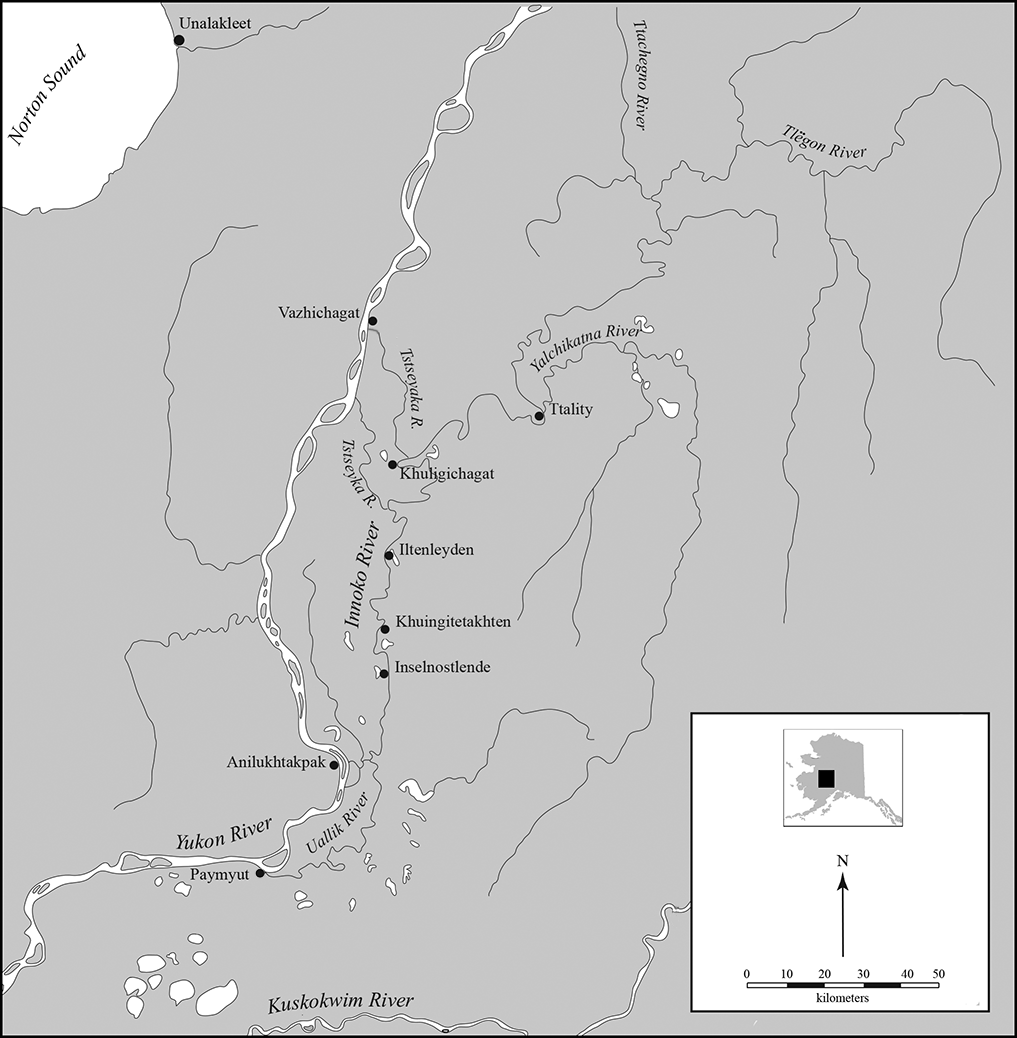
\includegraphics[width=\textwidth]{figures/pratt-fig3.png}
    \caption{Innoko River Area with Selected (Zagoskin) Place Names }
    \label{pratt-fig3}
\end{figure}

\clearpage
\begin{figure}[h]
    \centering
    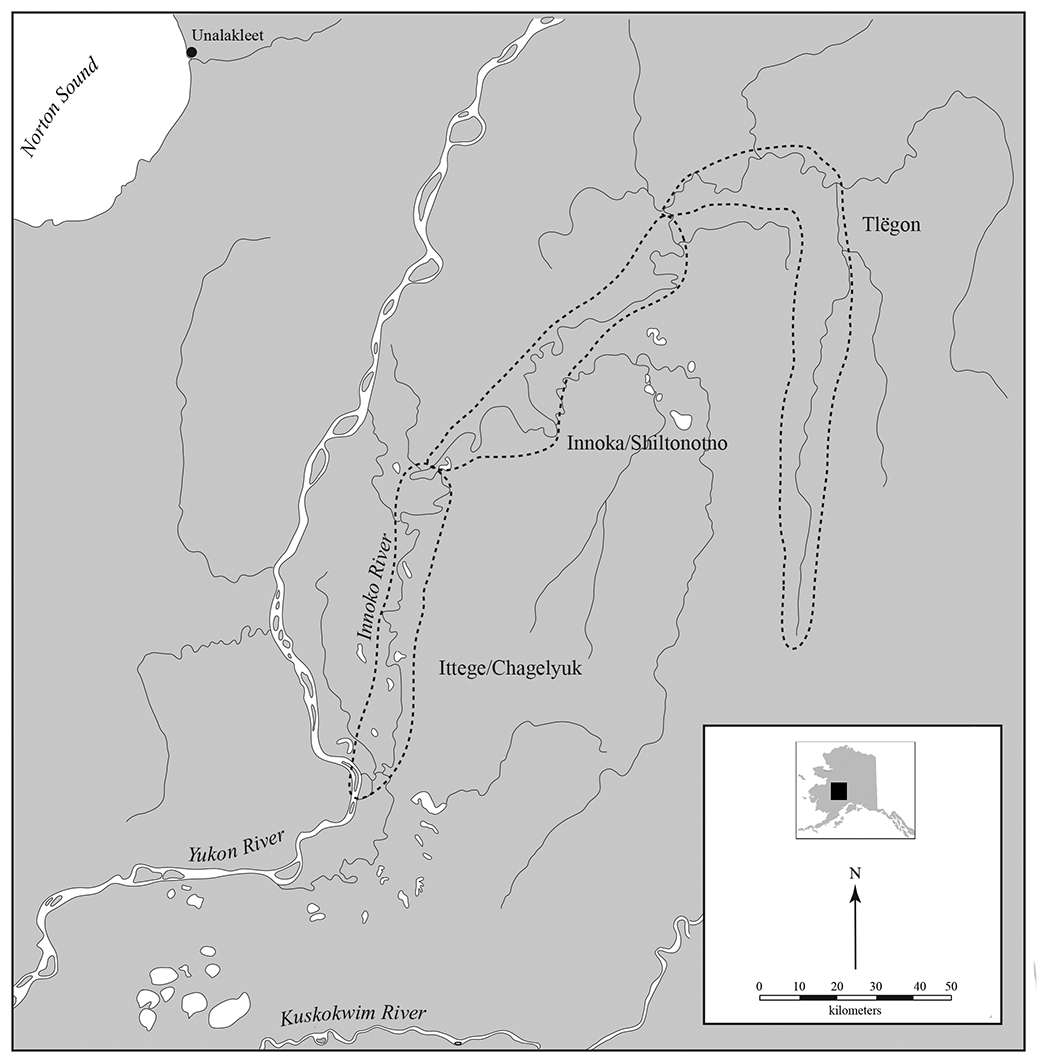
\includegraphics[width=\textwidth]{figures/pratt-fig4.png}
    \caption{Three Named Sections of the Innoko River Drainage Reported by Zagoskin}
    \label{pratt-fig4}
\end{figure}

\clearpage
\begin{figure}[h]
    \centering
    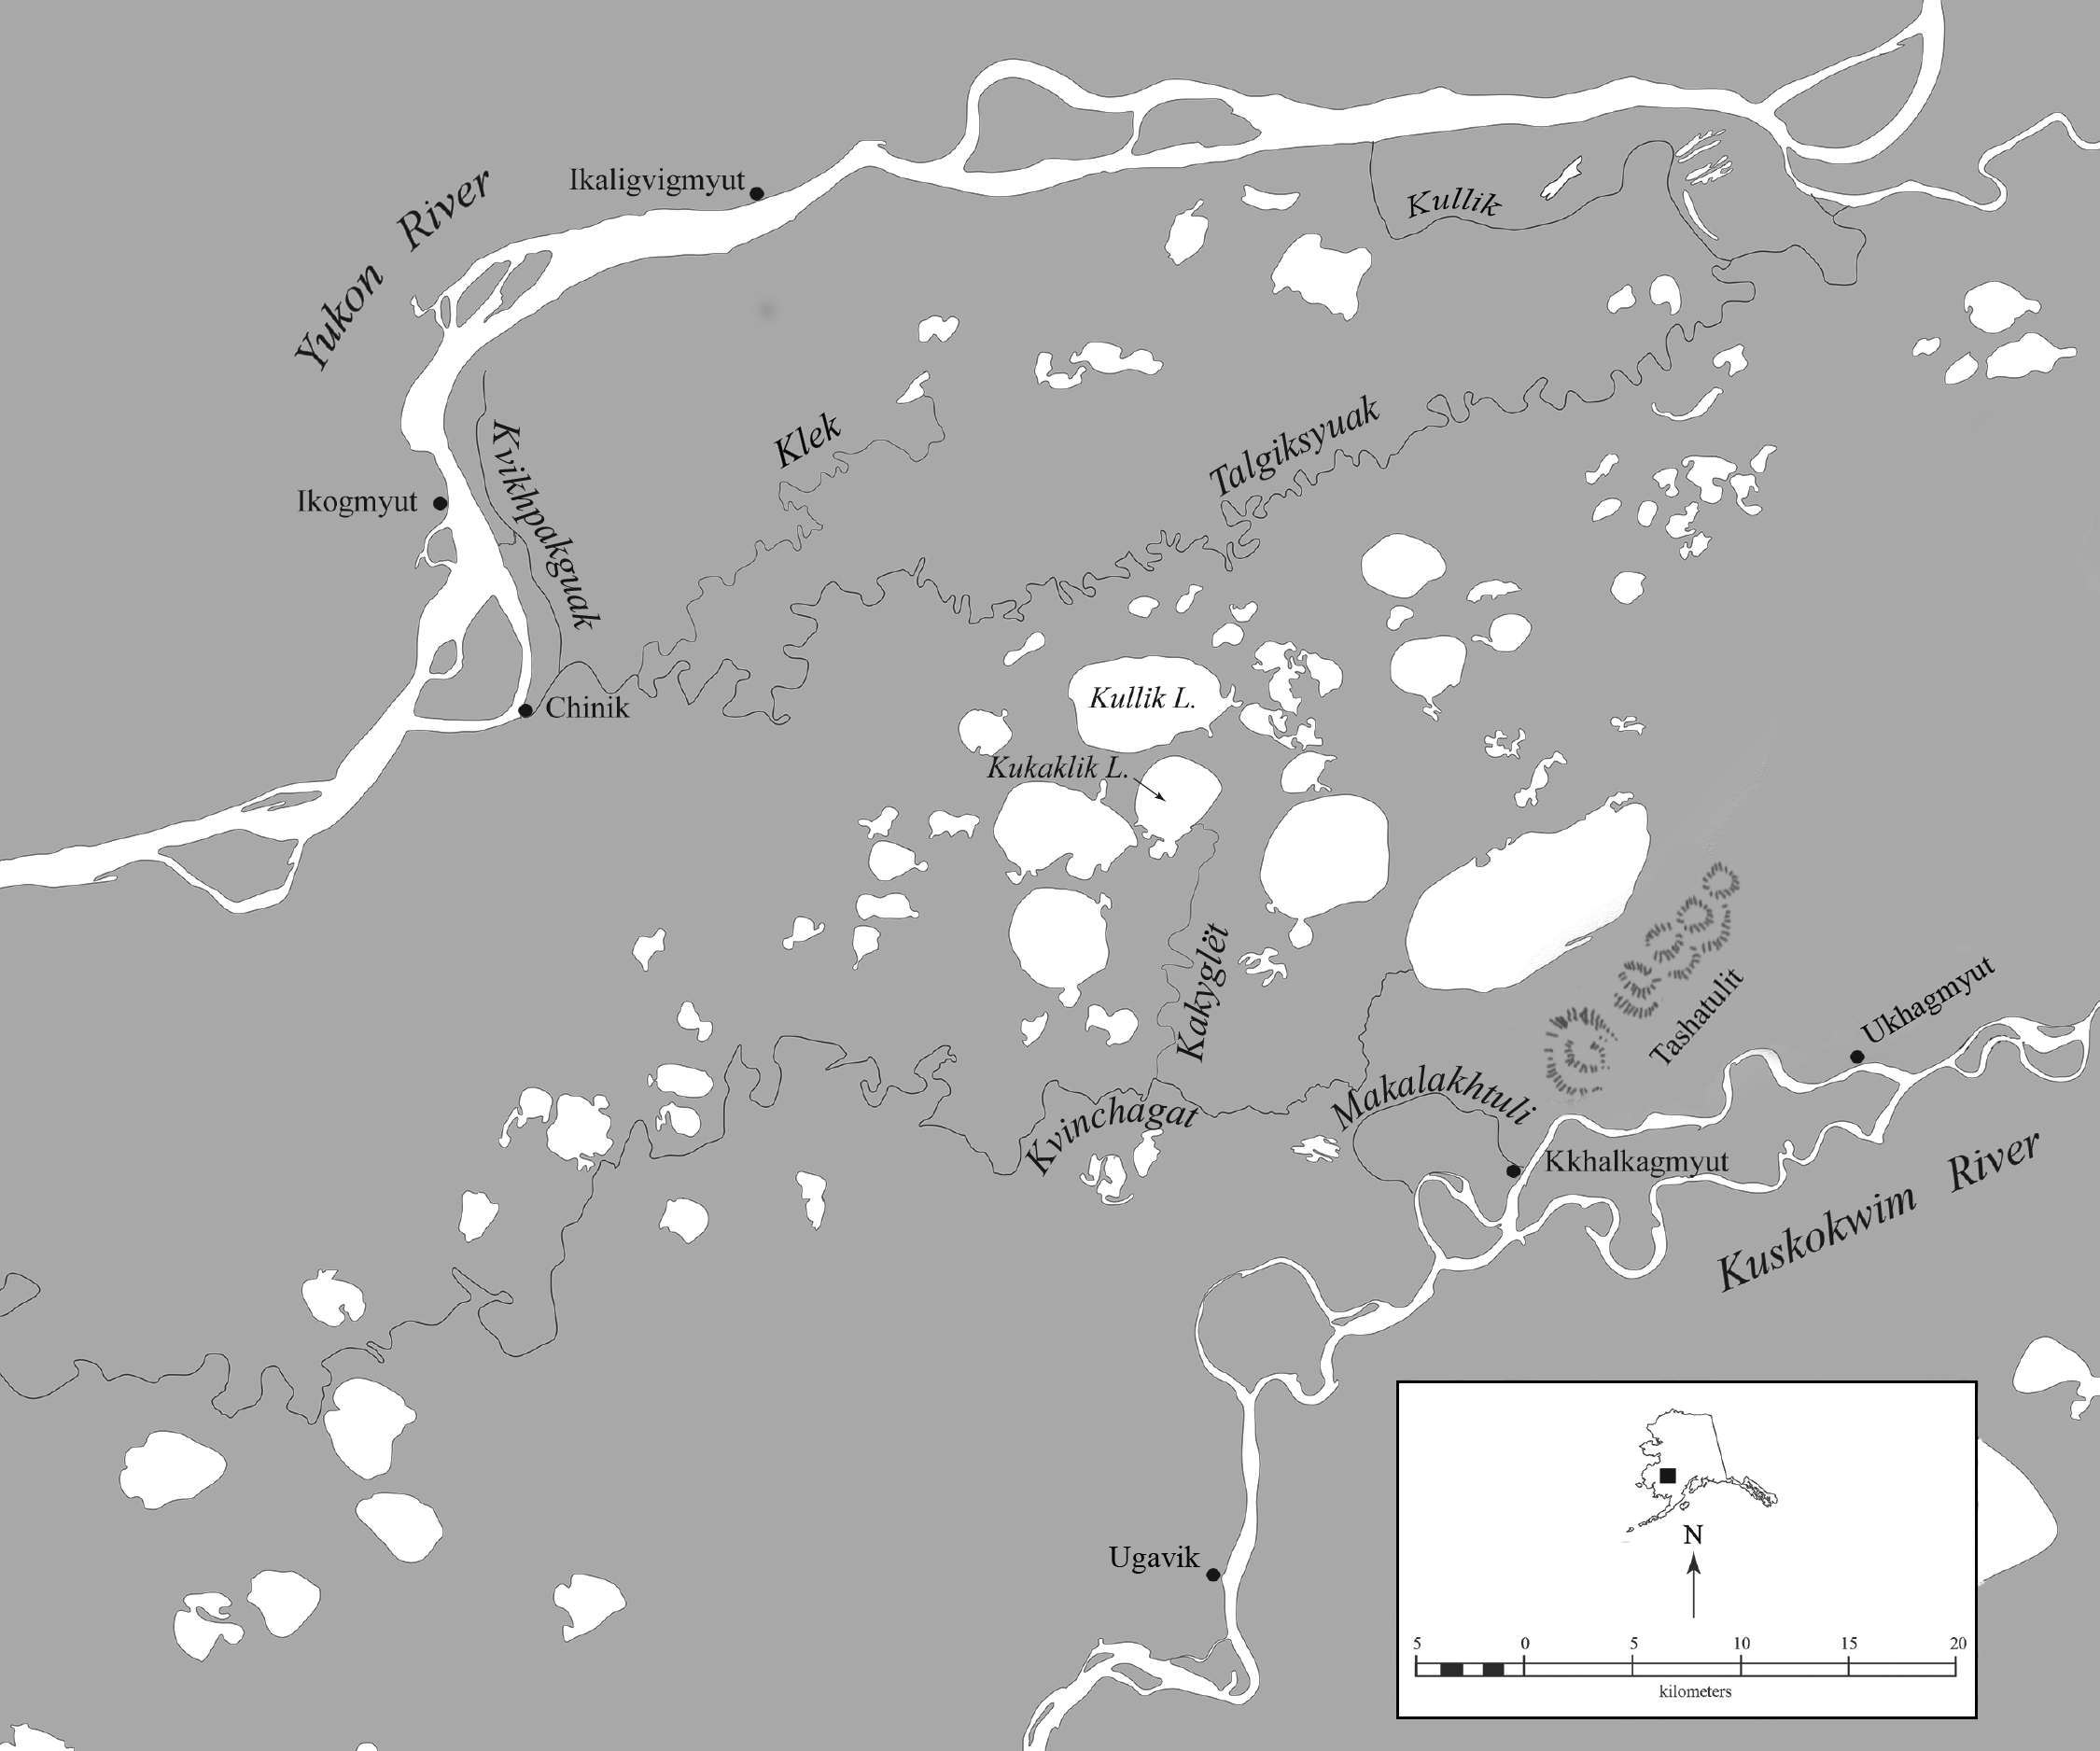
\includegraphics[width=\textwidth]{figures/pratt-fig5.png}
\caption{Yukon-Kuskokwim Portage Area with Selected Place Names Reported by Zagoskin. Map by Dale C. Slaughter.}
\label{pratt-fig5}[h]
\end{figure}

\clearpage
\begin{figure}[h]
    \centering
    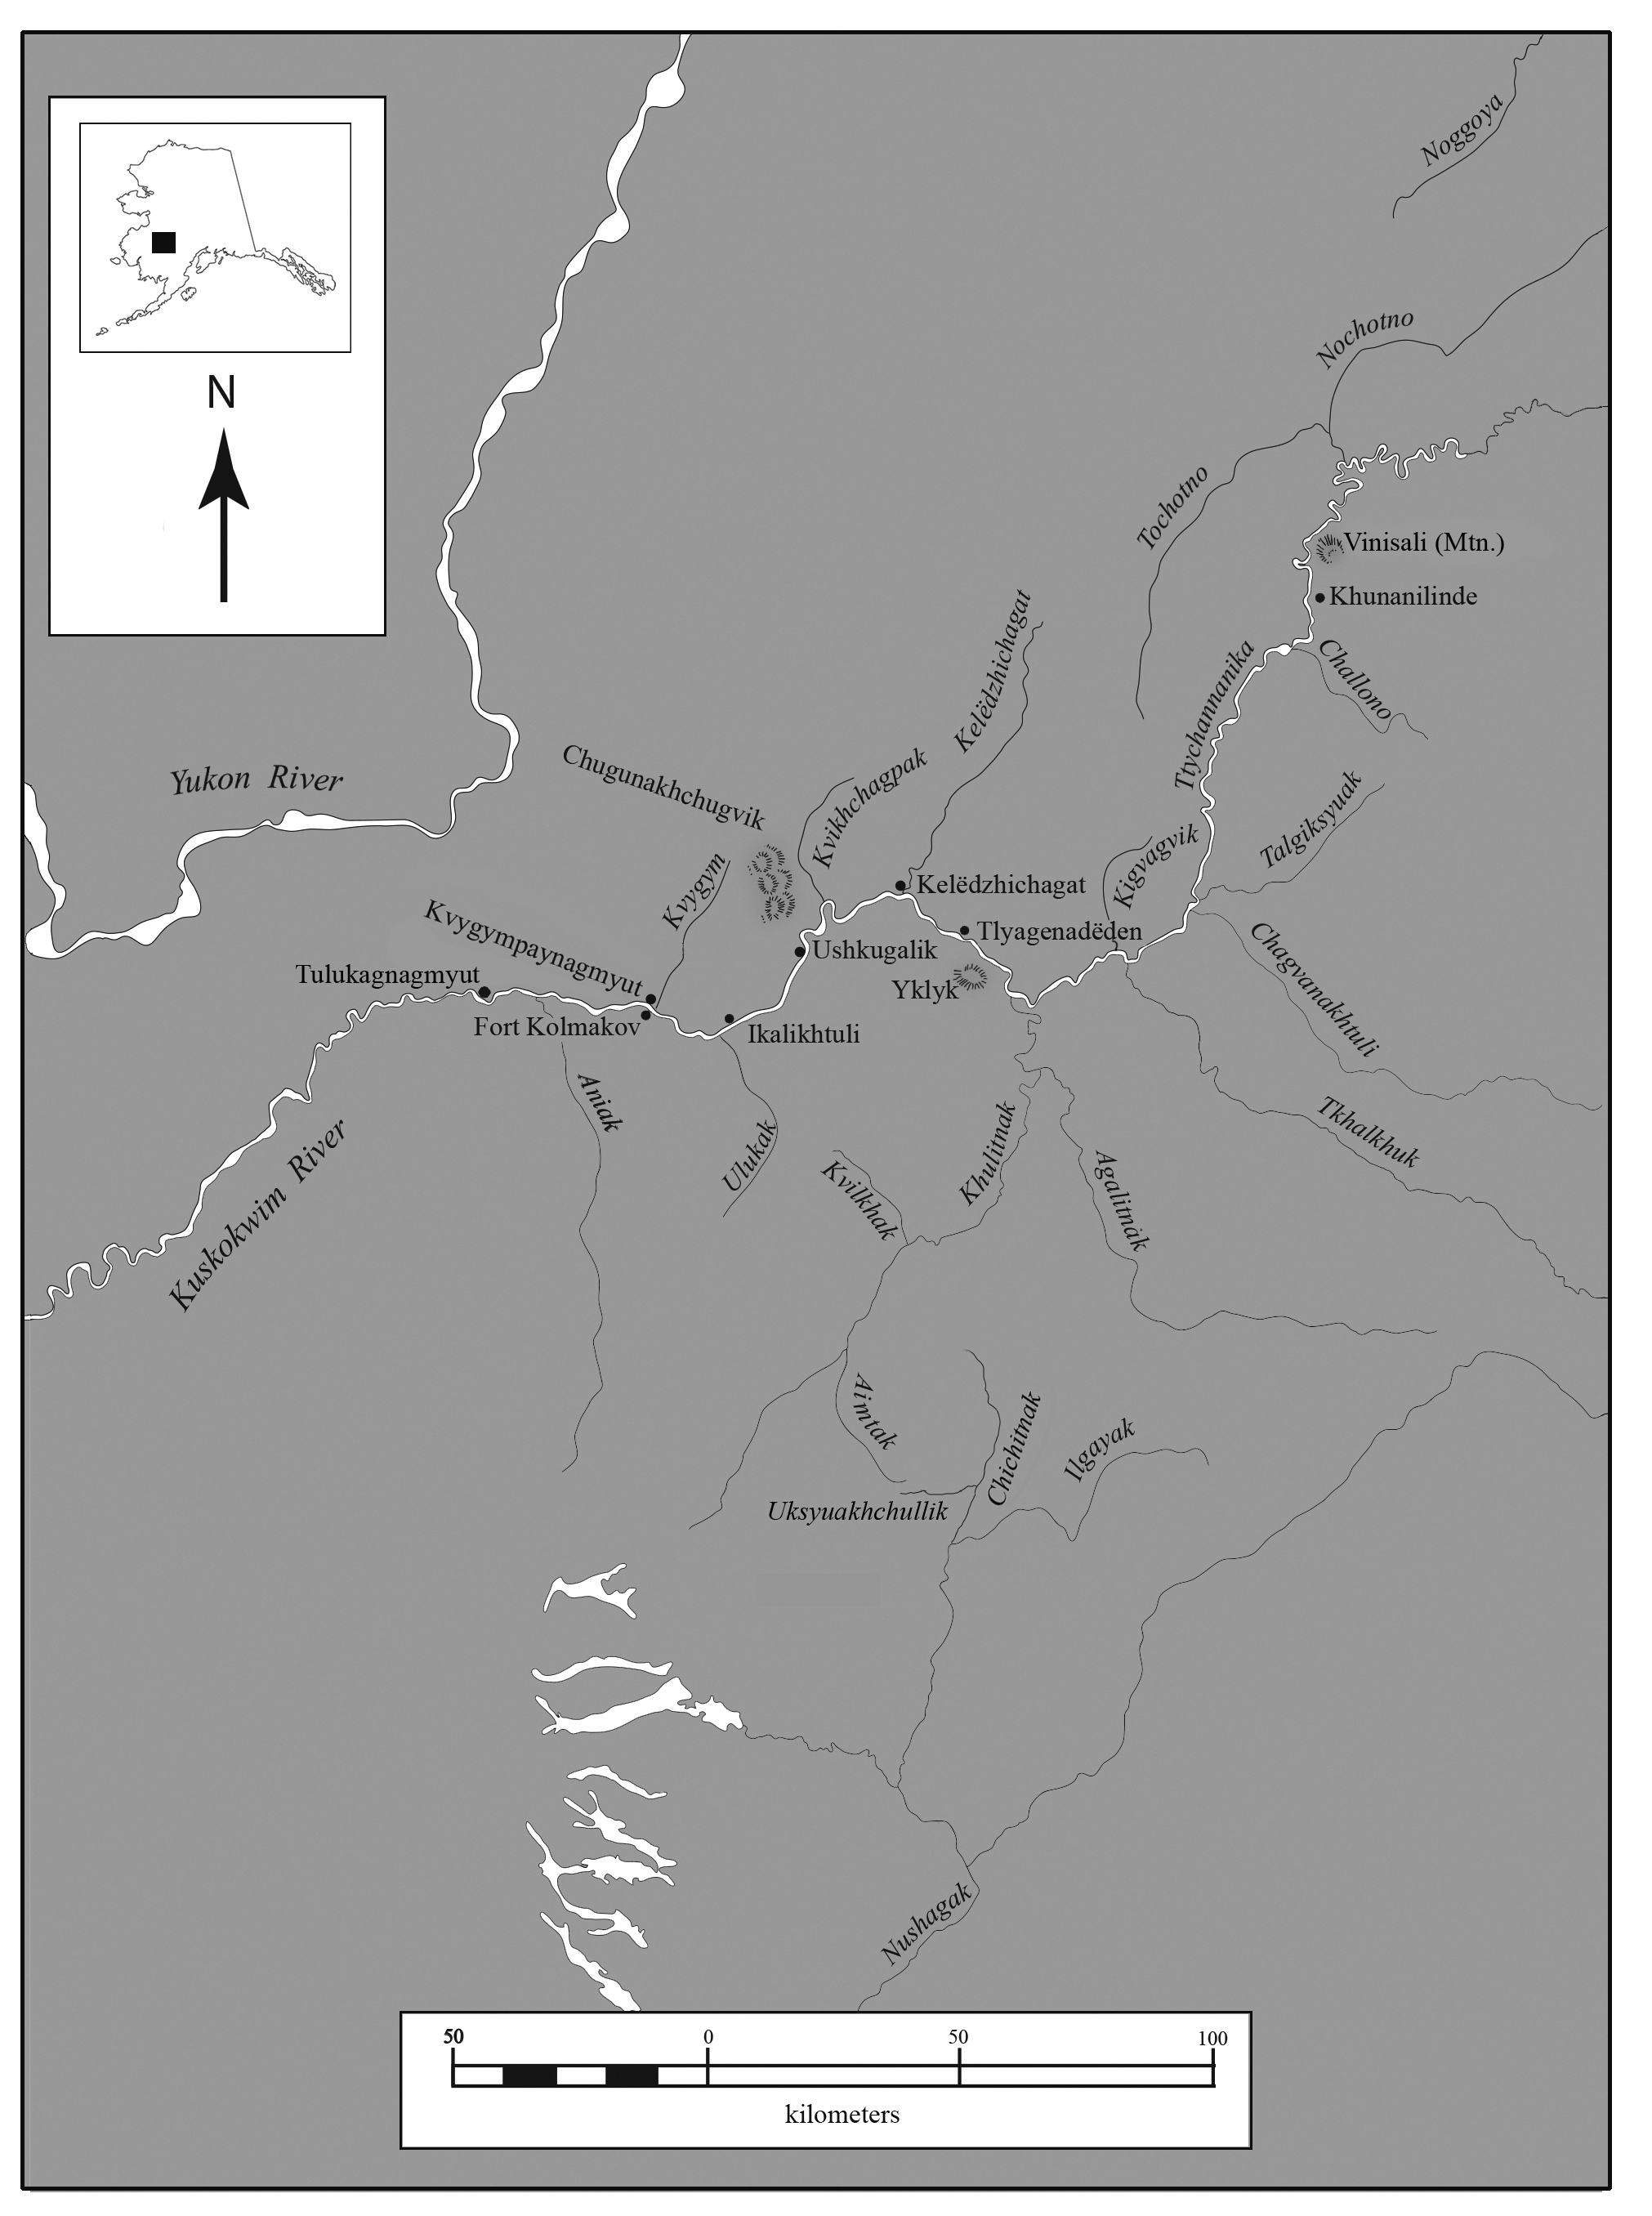
\includegraphics[width=\textwidth]{figures/pratt-fig6.png}
\caption{Middle Kuskokwim River Area with Selected Place Names Reported by Zagoskin. Map by Dale C. Slaughter.}
\label{pratt-fig6}
\end{figure}

%%%%%%%%%%%%% end appendix %%%%%%%%%%%%%%%%%%%%%







\label{pratt-ch-end}
